\chapter{Svolgimento dello \textit{stage}} 
\label{cap:descrizione-stage}

\section{Flusso di lavoro}
\subsection{Pianificazione delle attività}
In accordo agli obiettivi descritti in \ref{sec:obiettiviStage}, ho redatto, insieme al \textit{tutor} aziendale, una pianficazione settimanale delle attività da svolgere.
Nella tabella \ref{tab:prevAttività} presento la pianificazione di tali attività.

\renewcommand{\arraystretch}{1.5}
\begin{longtable}{|p{3cm}|p{9cm}|} 
    \hline
    \rowcolor{tableheader}\textbf{Periodo} & \textbf{Descrizione attività} \\
    \hline
    \endfirsthead

    \rowcolor{tableheader}\textbf{Periodo} & \textbf{Descrizione attività} \\
    \hline
    \endhead

    \hline
    \endfoot

    \hline
    \endlastfoot
    \rowcolor{tableevenrow} Prima settimana  & \begin{tabular}[t]{@{}p{9cm}@{}}
        - Studio ed apprendimento delle tecnologie di sviluppo \\
        - Definizione delle \textit{user stories} \\
    \end{tabular} \\
    \hline
    \hline
    \rowcolor{tableoddrow} Seconda settimana  &  \begin{tabular}[t]{@{}p{9cm}@{}}
        - Creazione \textit{ticket} di \textit{mock} \\
        - Caricamento dei \textit{ticket} all'interno dell'\gls{its} Jira
    \end{tabular} \\
    \hline
    \rowcolor{tableevenrow} Terza settimana & \begin{tabular}[t]{@{}p{9cm}@{}}
        - Reperire i ticket completati da Jira\\
        - Salvataggio \textit{ticket} su \textit{database} MongoDB \\
        - Aggiornamento costante del \textit{database}\\
    \end{tabular} \\
    \hline
    \rowcolor{tableoddrow} Quarta settimana & \begin{tabular}[t]{@{}p{9cm}@{}}
        - Studio \gls{embedding-g} per \gls{rag}\\
        - \gls{tokenizzazioneg}, ovvero la divisione del testo in unità che l'\gls{llm} elabora, dei \textit{ticket} contenuti nel \textit{database} MongoDB \\
        - Connessione tra AWS Bedrock e MongoDB per \gls{rag-g}\\
    \end{tabular} \\
    \hline
    \rowcolor{tableevenrow} Quinta settimana & \begin{tabular}[t]{@{}p{9cm}@{}}
        - Creazione di domande di \textit{benchmark}\\
        - Confronto tra i diversi \gls{llm}, modelli progettati per generare testo umano\\
    \end{tabular} \\
    \hline
    \rowcolor{tableoddrow} Sesta settimana & \begin{tabular}[t]{@{}p{9cm}@{}}
        - Aggiornamento del \textit{ticket} Jira con la proposta di risoluzione, generata tramite il sistema di IA Generativa\\
        - Sviluppo di un \textit{chatbot} per l'interrogazione sui \textit{ticket} Jira\\
    \end{tabular} \\ 
    \hline
    \rowcolor{tableevenrow} Settima settimana & \begin{tabular}[t]{@{}p{9cm}@{}}
        - Migliorie al sistema di proposte di risoluzione Jira\\
        - Migliorie al \textit{chatbot}, dando all'utente la possibilità di utilizzare \gls{llm} diversi \\
        - Implementare un sistema di autenticazione nel \textit{chatbot} \\
    \end{tabular} \\ 
    \hline
    \rowcolor{tableoddrow} Ottava settimana & \begin{tabular}[t]{@{}p{9cm}@{}}
        - Realizzazione di una presentazione sui progetti sviluppati\\
        - Redazione documento manuale utente \\
        - Redazione documento sull'architettura e sulle scelte progettuali adottate \\
        - Miglioria al \textit{chatbot} per proposte di risoluzione più descrittive \\
    \end{tabular} \\ 
    \hline
    \caption{Pianificazione del progetto di \textit{stage}}
    \label{tab:prevAttività}
\end{longtable}
\noindent
Qui di seguito presento nell'immagine \ref{fig:gantt} che rappresenta la pianificazione delle attività svolte durante il periodo di \textit{stage} tramite un diagramma di Gantt.
\begin{figure}[H]
    \centering
    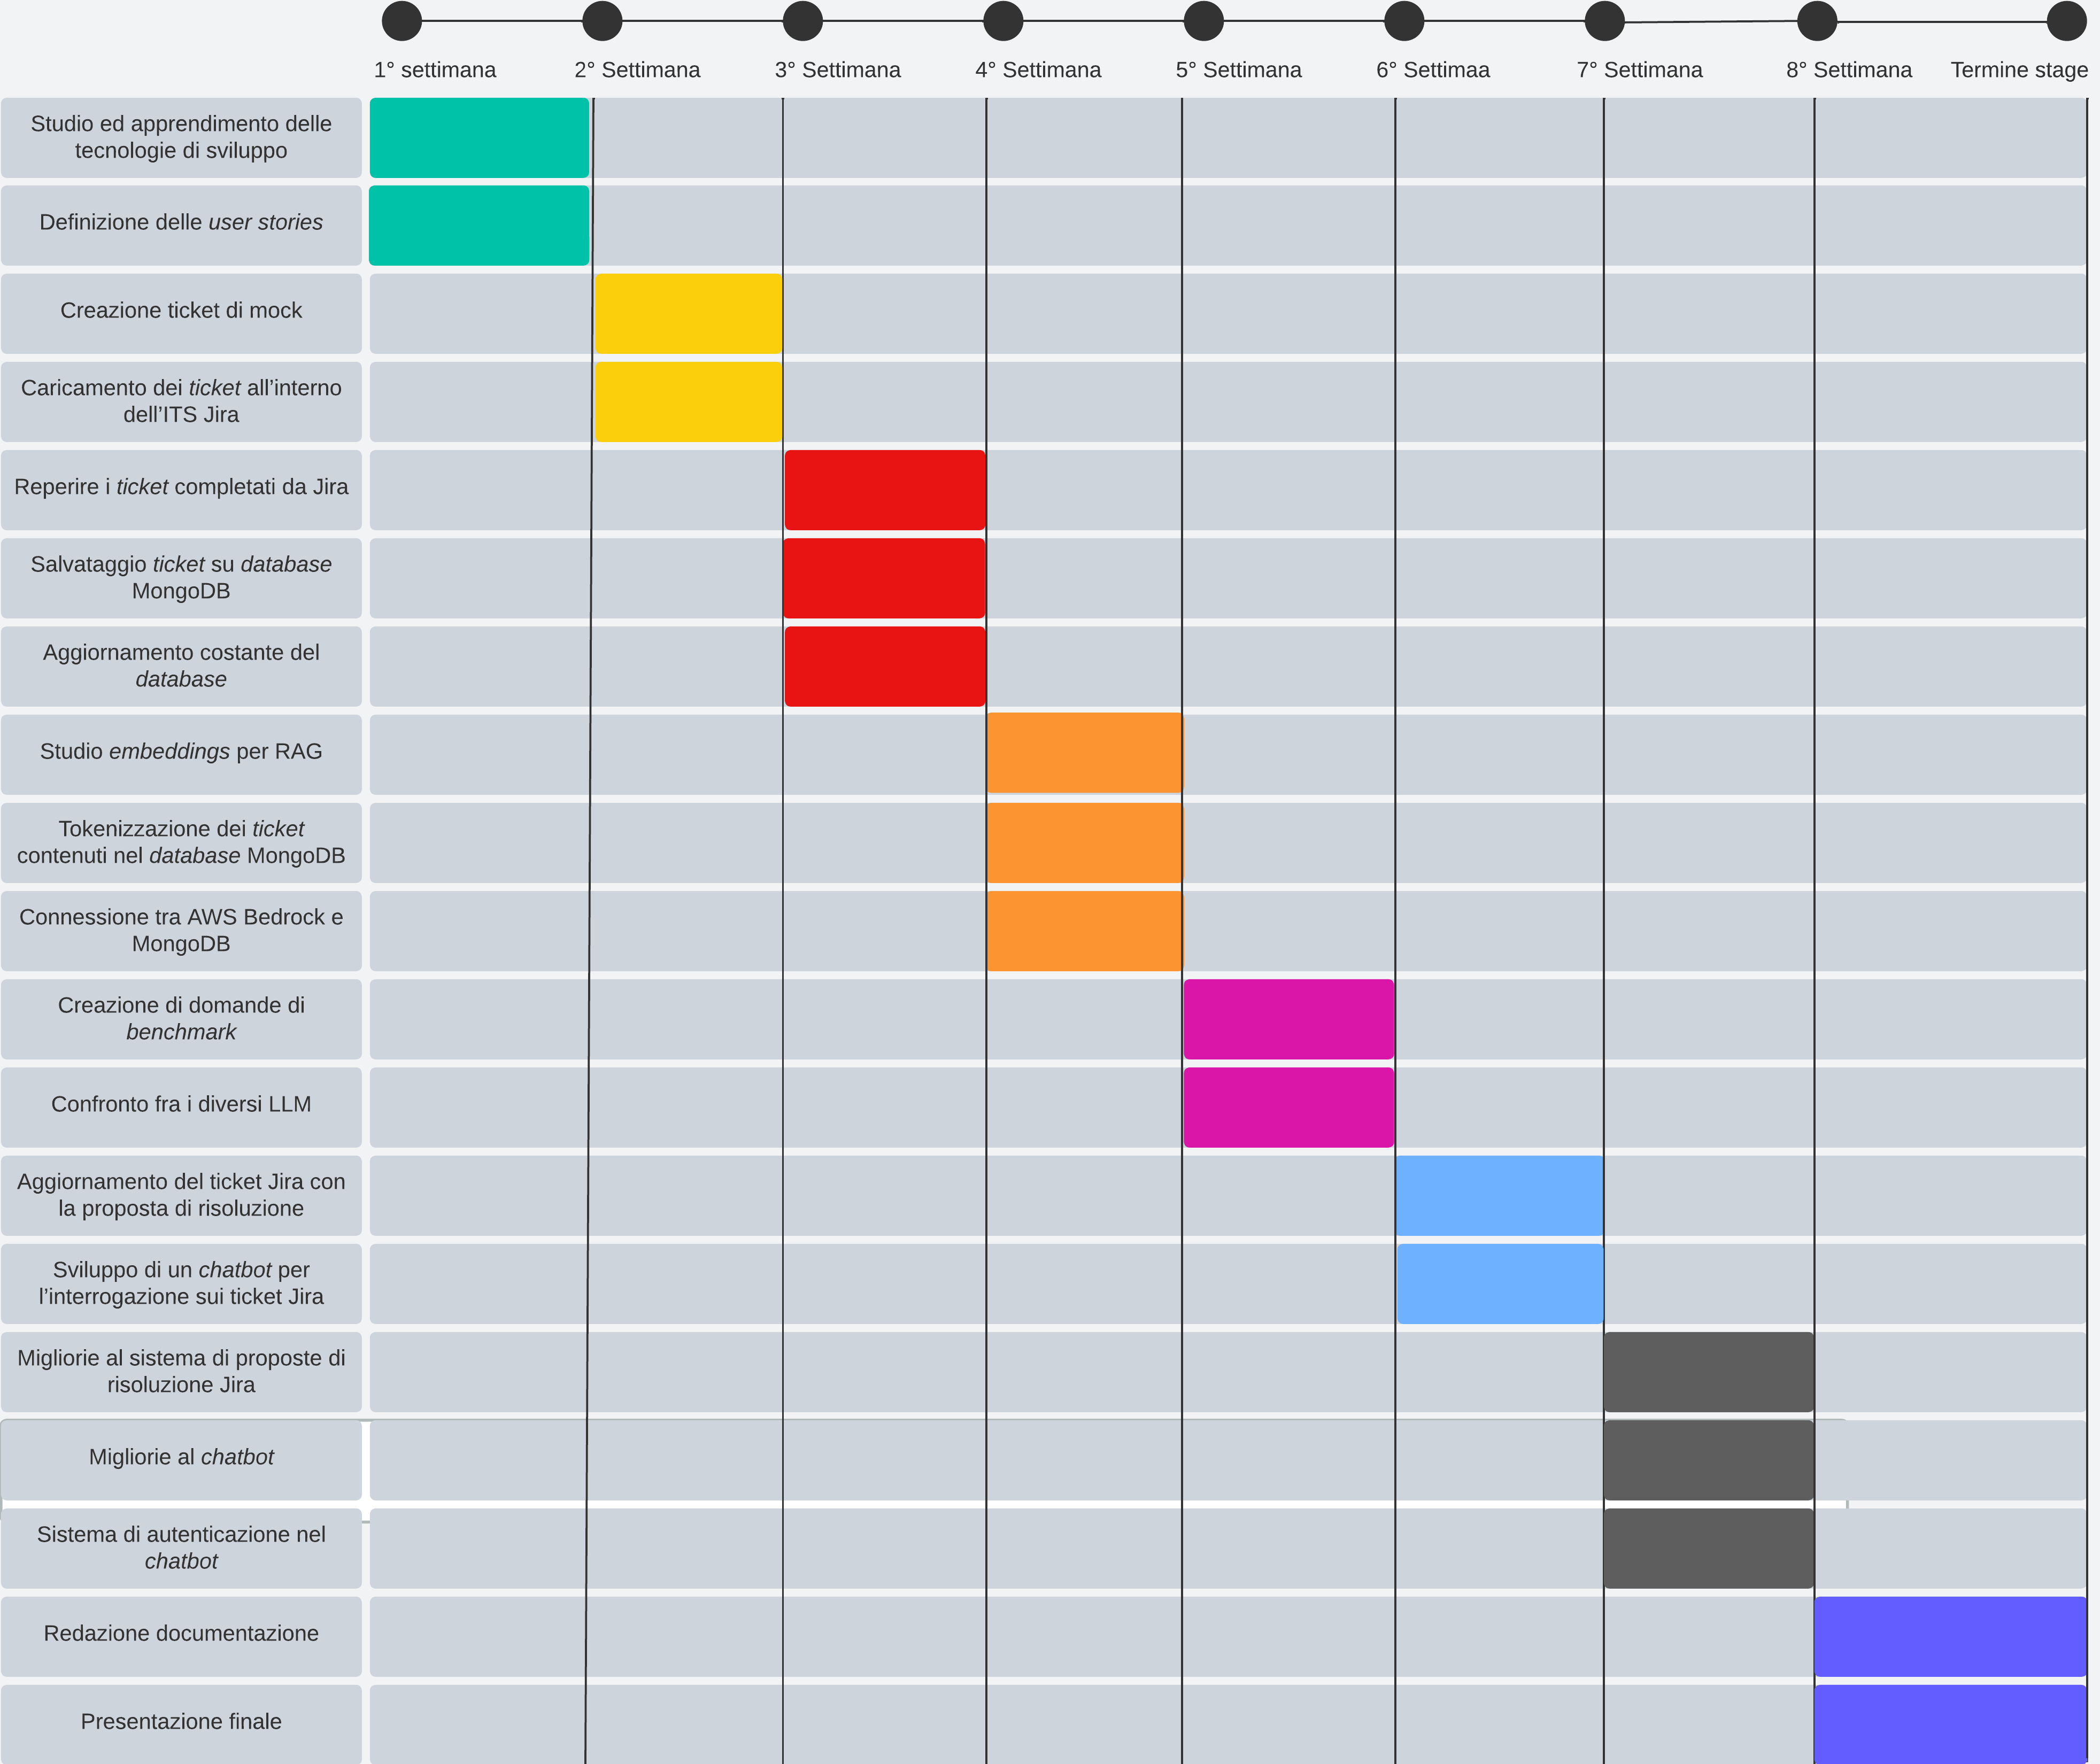
\includegraphics[width=1\textwidth]{diagrammaGantt.png}
    \caption{Diagramma di Gantt delle attività svolte durante lo \textit{stage}}
    \label{fig:gantt}
\end{figure}

\subsection{Revisioni di progetto} \label{sec:revisioni}
L'attività di revisione del progetto ritengo essere stata di fondamentale importanza e utile ai fini formativi dello \textit{stage}.
Nel corso del tirocinio ho avuto modo di sperimentare due tipologie di revisione: il \textit{daily}, un incontro giornaliero con il \textit{tutor} aziendale, e lo \textit{sprint review}, un incontro settimanale con il \textit{tutor} aziendale per valutare quanto e cosa avevo svolto durante la settimana e per pianificare le attività per la settimana successiva.
L'occorrenza del \textit{daily} è stata purtroppo però limitata a causa di numerosi impegni che il \textit{tutor} aziendale aveva durante la giornata. Sono stati comunque utili, soprattutto all'inizio dello \textit{stage}, per chiarire dubbi su come procedere con le attività e per ricevere feedback immediato su quanto svolto.
Lo \textit{sprint review} invece è stato quello presente con regolarità durante tutto il periodo di \textit{stage}, che mi ha permesso di ricevere un feedback più dettagliato su quanto avevo svolto durante la settimana. Questi incontri periodici mi hanno permesso di correggere eventuali errori e di migliorare la qualità del lavoro svolto.

\subsection{Interazioni con il tutor aziendale}
Come descritto nella sezione \ref{sec:revisioni}, le interazioni con il \textit{tutor} aziendale sono state numerose e di fondamentale importanza per il corretto svolgimento delle attività.
Nelle giornate in cui non era possibile riferirmi direttamente al \textit{tutor} aziendale, mi sono rivolto ad una figura di supporto, che in caso di assenza o indisponibilità del \textit{tutor} aziendale, era predista all'aiuto degli stagisti in caso di problematiche.


\section{Analisi dei rischi} \label{sec:rischi}
I primi giorni di stage sono stati dedicati all'individuazione dei potenziali rischi che avrei potuto incontrare durante lo svolgimento dello \textit{stage}.
Si farà riferimento ai rischi individuati seguendo la seguente notazione: 
\begin{center}
    \textbf{R-[Tipologia]-[Probabilità][Impatto]-[Indice]}
\end{center}
dove:
\begin{itemize}
    \item \textbf{R}: abbreviazione di Rischio
    \item \textbf{Tipologia}: \\ Natura del rischio: \begin{itemize}
        \item \textbf{T}: Tecnologico
        \item \textbf{O}: Organizzativo
        \item \textbf{P}: Personale
    \end{itemize}
    \item \textbf{Probabilità}: \\ Numero intero positivo che indica la probabilità di occorrenza del rischio: \begin{itemize}
        \item \textbf{1}: Alta
        \item \textbf{2}: Media
        \item \textbf{3}: Bassa
    \end{itemize}
    \item \textbf{Impatto}: \\ Valore alfabetico che indica la probabilità di occorrenza del rischio: \begin{itemize}
        \item \textbf{A}: Alto
        \item \textbf{B}: Medio
        \item \textbf{C}: Basso
    \end{itemize}
    \item \textbf{Indice}: Numero intero positivo incrementale che determina univocamente il rischio relativamente ad una specifica tipologia
\end{itemize}

\renewcommand{\arraystretch}{1.5}
\begin{longtable}{|p{3cm}|p{4.3cm}|p{4.5cm}|} 
    \hline
    \rowcolor{tableheader}\textbf{Codice} & \textbf{Descrizione} & \textbf{Mitigazione} \\
    \hline
    \endfirsthead

    \rowcolor{tableheader}\textbf{Codice} & \textbf{Descrizione} & \textbf{Mitigazione} \\
    \hline
    \endhead

    \hline
    \endfoot

    \hline
    \endlastfoot

    \rowcolor{tableevenrow} R-T-1A-1 & Complessità del contesto di uso di servizi di IA Generativa & 
    Chiedere supporto al \textit{tutor} aziendale sul corretto utilizzo dei servizi di IA Generativa che verranno utilizzati \\
    \hline
    \rowcolor{tableoddrow} R-T-2B-2 & Complessità del contesto di sviluppo e attività di integrazione con la \textit{suite} Atlassian & 
    \begin{tabular}[t]{@{}p{4.3cm}@{}}
        - Riferimento a documentazione più dettagliata \\
        - Supporto da parte del \textit{tutor} aziendale \\
    \end{tabular} \\
    \hline
    \rowcolor{tableevenrow} R-T-1A-3 & Ridotta conoscenza dei servizi cloud \gls{aws} & 
    \begin{tabular}[t]{@{}p{4.3cm}@{}}
        - Studio approfondito dei servizi \gls{aws} \\
        - Documentazione dettagliata dei servizi \gls{aws} \\
        - Supporto da parte del \textit{tutor} aziendale
    \end{tabular} \\
    \hline
    \rowcolor{tableoddrow} R-P-3C-1 & Assenze per motivi di salute o personali & 
    Avvisare per tempo il \textit{tutor} aziendale in caso di ritardi, in modo da aggiornare la pianificazione delle attività \\
    \hline
    \rowcolor{tableevenrow} R-O-2A-1 & Lo sviluppo del progetto potrebbe non essere portato a termine nel periodo pianificato a causa di ritardi & 
    Avvisare per tempo il \textit{tutor} aziendale in modo da pianificare le attività per recuperare i giorni di assenza \\
    \hline

    \caption{Analisi dei rischi}
    \label{tab:rischi}
\end{longtable}





\section{Analisi dei requisiti}
\subsection{Aspettative del committente}
In accordo agli obiettivi descritti in \ref{sec:obiettiviStage}, mi è stato richiesto di sviluppare, a seguito di uno studio di fattibilità, un sistema integrato su Jira che alla creazione di un nuovo \textit{ticket}, venisse generata una proposta di risoluzione in base ai \textit{ticket} completati in passato e salvati in un \textit{database} MongoDB.
Inoltre, mi è stato richiesto di sviluppare un \textit{chatbot} che permettesse all'utente di interrogare l'assistente virtuale sui \textit{ticket} Jira e di ricevere proposte di risoluzione.

\subsection{Casi d'uso}
I diagrammi dei casi d'uso permettono di descrivere le interazione tra gli attori e il sistema.  
La convezione che ho utilizzato per la stesura dei casi d'uso è stata la seguente:
\begin{center}
    \textbf{{UC[Numero]}: nome del caso d'uso}
\end{center}
\begin{itemize}
    \item \textbf{UC}: acronimo di \textit{Use Case};
    \item \textbf{Numero}: numero progressivo del caso d'uso. I sottocasi vengono rappresentati nella forma [Numero].[SottoNumero];
\end{itemize}
a cui ho associato una descrizione, la lista degli attori coinvolti, le precondizioni e le postcondizioni affinche il caso d'uso possa avvenire.
Per riassumere i casi d'uso, sono presenti dei diagrammi \gls{umlg} per una rappresentazione grafica degli scenari. Verrano presentati i diagrammi dei casi d'uso principali e non banali dei progetti.
\subsubsection{Attori}
Nel contesto dei casi d'uso, con un attore si definisce chi o cosa interagisce con la specifica funzionalità descritta dal caso d'uso.
Gli attori che ho individuato si suddividono in 2 categorie:
\begin{itemize}
    \item \textbf{Attori principali} \begin{itemize} \item \textbf{Utente generico}: utente che non ha effettuato l'autenticazione nel sistema e nel \textit{chatbot}. Ha accesso unicamente alla pagina di \textit{login}; \item \textbf{Utente amministratore}: utente che ha effettuato l'autenticazione. Ha accesso a tutte le funzionalità del sistema.
    \end{itemize}
    \item \textbf{Attori secondari}: \begin{itemize} \item \textbf{\gls{llm}}: è un attore secondario che permette la generazione di \gls{embedding-g} e di generazione di testo tramite modelli di linguaggio. Questo attore a sua volta può essere interpretato da AmazonTitanV2 (modello di generazione di \gls{embedding-g} offerto da \gls{aws} Bedrock) e da Claude3.5Sonnet (\gls{llm} offerto da \gls{aws} Bedrock).
    \end{itemize}
\end{itemize}
\begin{figure}[H]
    \centering
    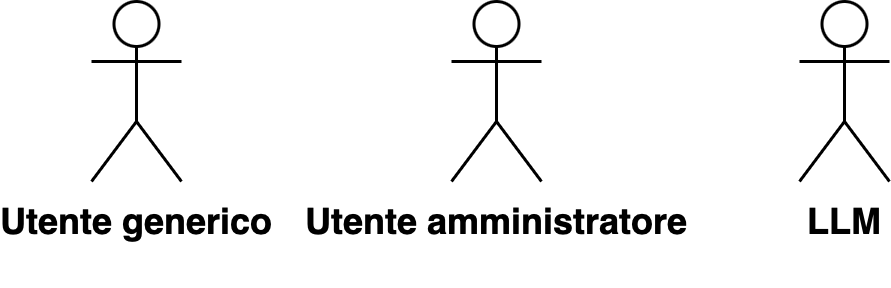
\includegraphics[width=0.55\textwidth]{actors.png}
    \caption{Attori dei casi d'uso}
    \label{fig:attori}
\end{figure}
\subsection*{Lista dei casi d'uso}
\subsubsection{Sistema di proposte di risoluzione Jira}
\subsubsection{UC0: Creazione di un nuovo ticket}
\textbf{Attori principali}: Utente amministratore \\
\textbf{Precondizioni}: L'utente amministratore è autenticato nel \textit{workspace} Jira\\
\textbf{Descrizione}: L'utente amministratore crea un nuovo \textit{ticket} all'interno del progetto Jira \\
\textbf{Postcondizioni}: Il \textit{ticket} è stato creato \\
\begin{figure}[H]
    \centering
    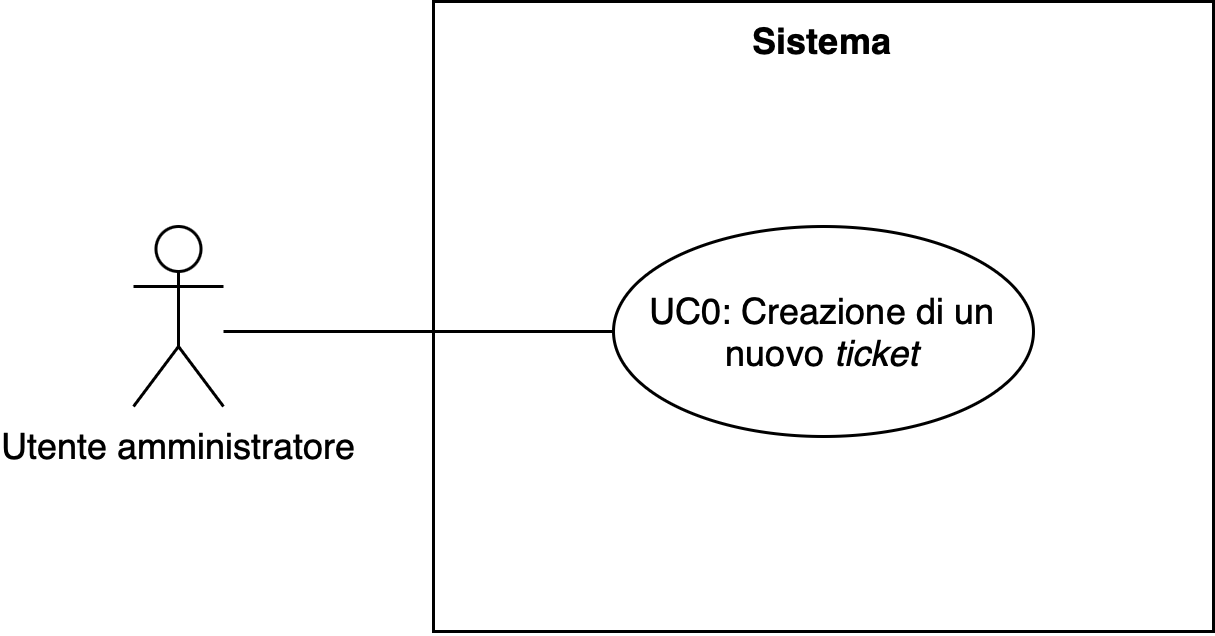
\includegraphics[width=0.55\textwidth]{uc0.png}
    \caption{Diagramma del caso d'uso UC0}
    \label{fig:UC0}
\end{figure}
\subsubsection{UC1: Richiesta proposta di risoluzione}
\textbf{Attori principali}: Utente amministratore \\
\textbf{Precondizioni}: L'utente amministratore ha creato un nuovo \textit{ticket} \\
\textbf{Descrizione}: Viene richiesto al sistema di generare una proposta di risoluzione per il \textit{ticket} appena creato \\
\textbf{Postcondizioni}: Il sistema inizia il processo di generazione della proposta di risoluzione \\

\subsubsection{UC1.1: Generazione \gls{embedding-g} del ticket}
\textbf{Attori principali}: \gls{llm} \\
\textbf{Precondizioni}: Il \textit{ticket} è stato creato ed è stata richiesta una proposta di risoluzione \\
\textbf{Descrizione}: Viene richiesto all'\gls{llm} di generare l'\gls{embedding-g} del \textit{ticket} per effettuare la ricerca dei \textit{ticket} completati più simili \\
\textbf{Postcondizioni}: L'\gls{embedding-g} del \textit{ticket} è stato generato \\

\subsubsection{UC1.2: Ricerca \textit{ticket} più simili}
\textbf{Attori principali}: Sistema \\ 
\textbf{Precondizioni}: È stato generato l'\gls{embedding-g} del \textit{ticket} creato\\
\textbf{Descrizione}: Il sistema effettua una ricerca vettoriale all'interno del \textit{database} con l'utilizzo dell'\gls{embedding-g}, per trovare i \textit{ticket} completati più simili al \textit{ticket} creato \\
\textbf{Postcondizioni}: I \textit{ticket} completati più simili vengono restuiti dal sistema \\

\subsubsection{UC1.3: Generazione proposta di risoluzione}
\textbf{Attori principali}: \gls{llm} \\
\textbf{Precondizioni}: Sono stati restituiti i \textit{ticket} completati più simili al \textit{ticket} creato \\
\textbf{Descrizione}: Viene richiesto all'\gls{llm} di generare una proposta di risoluzione per il \textit{ticket} creato usando come contesto i \textit{ticket} completati più simili \\
\textbf{Postcondizioni}: La proposta di risoluzione è stata generata ed inserita all'interno del campo adibito, del \textit{ticket} creato \\
\textbf{Estensioni}: \textbf{UC1.3.1}: I \textit{ticket} completati non sono inerenti al \textit{ticket} creato e non è possibile generare una proposta di risoluzione \\
\begin{figure}[H]
    \centering
    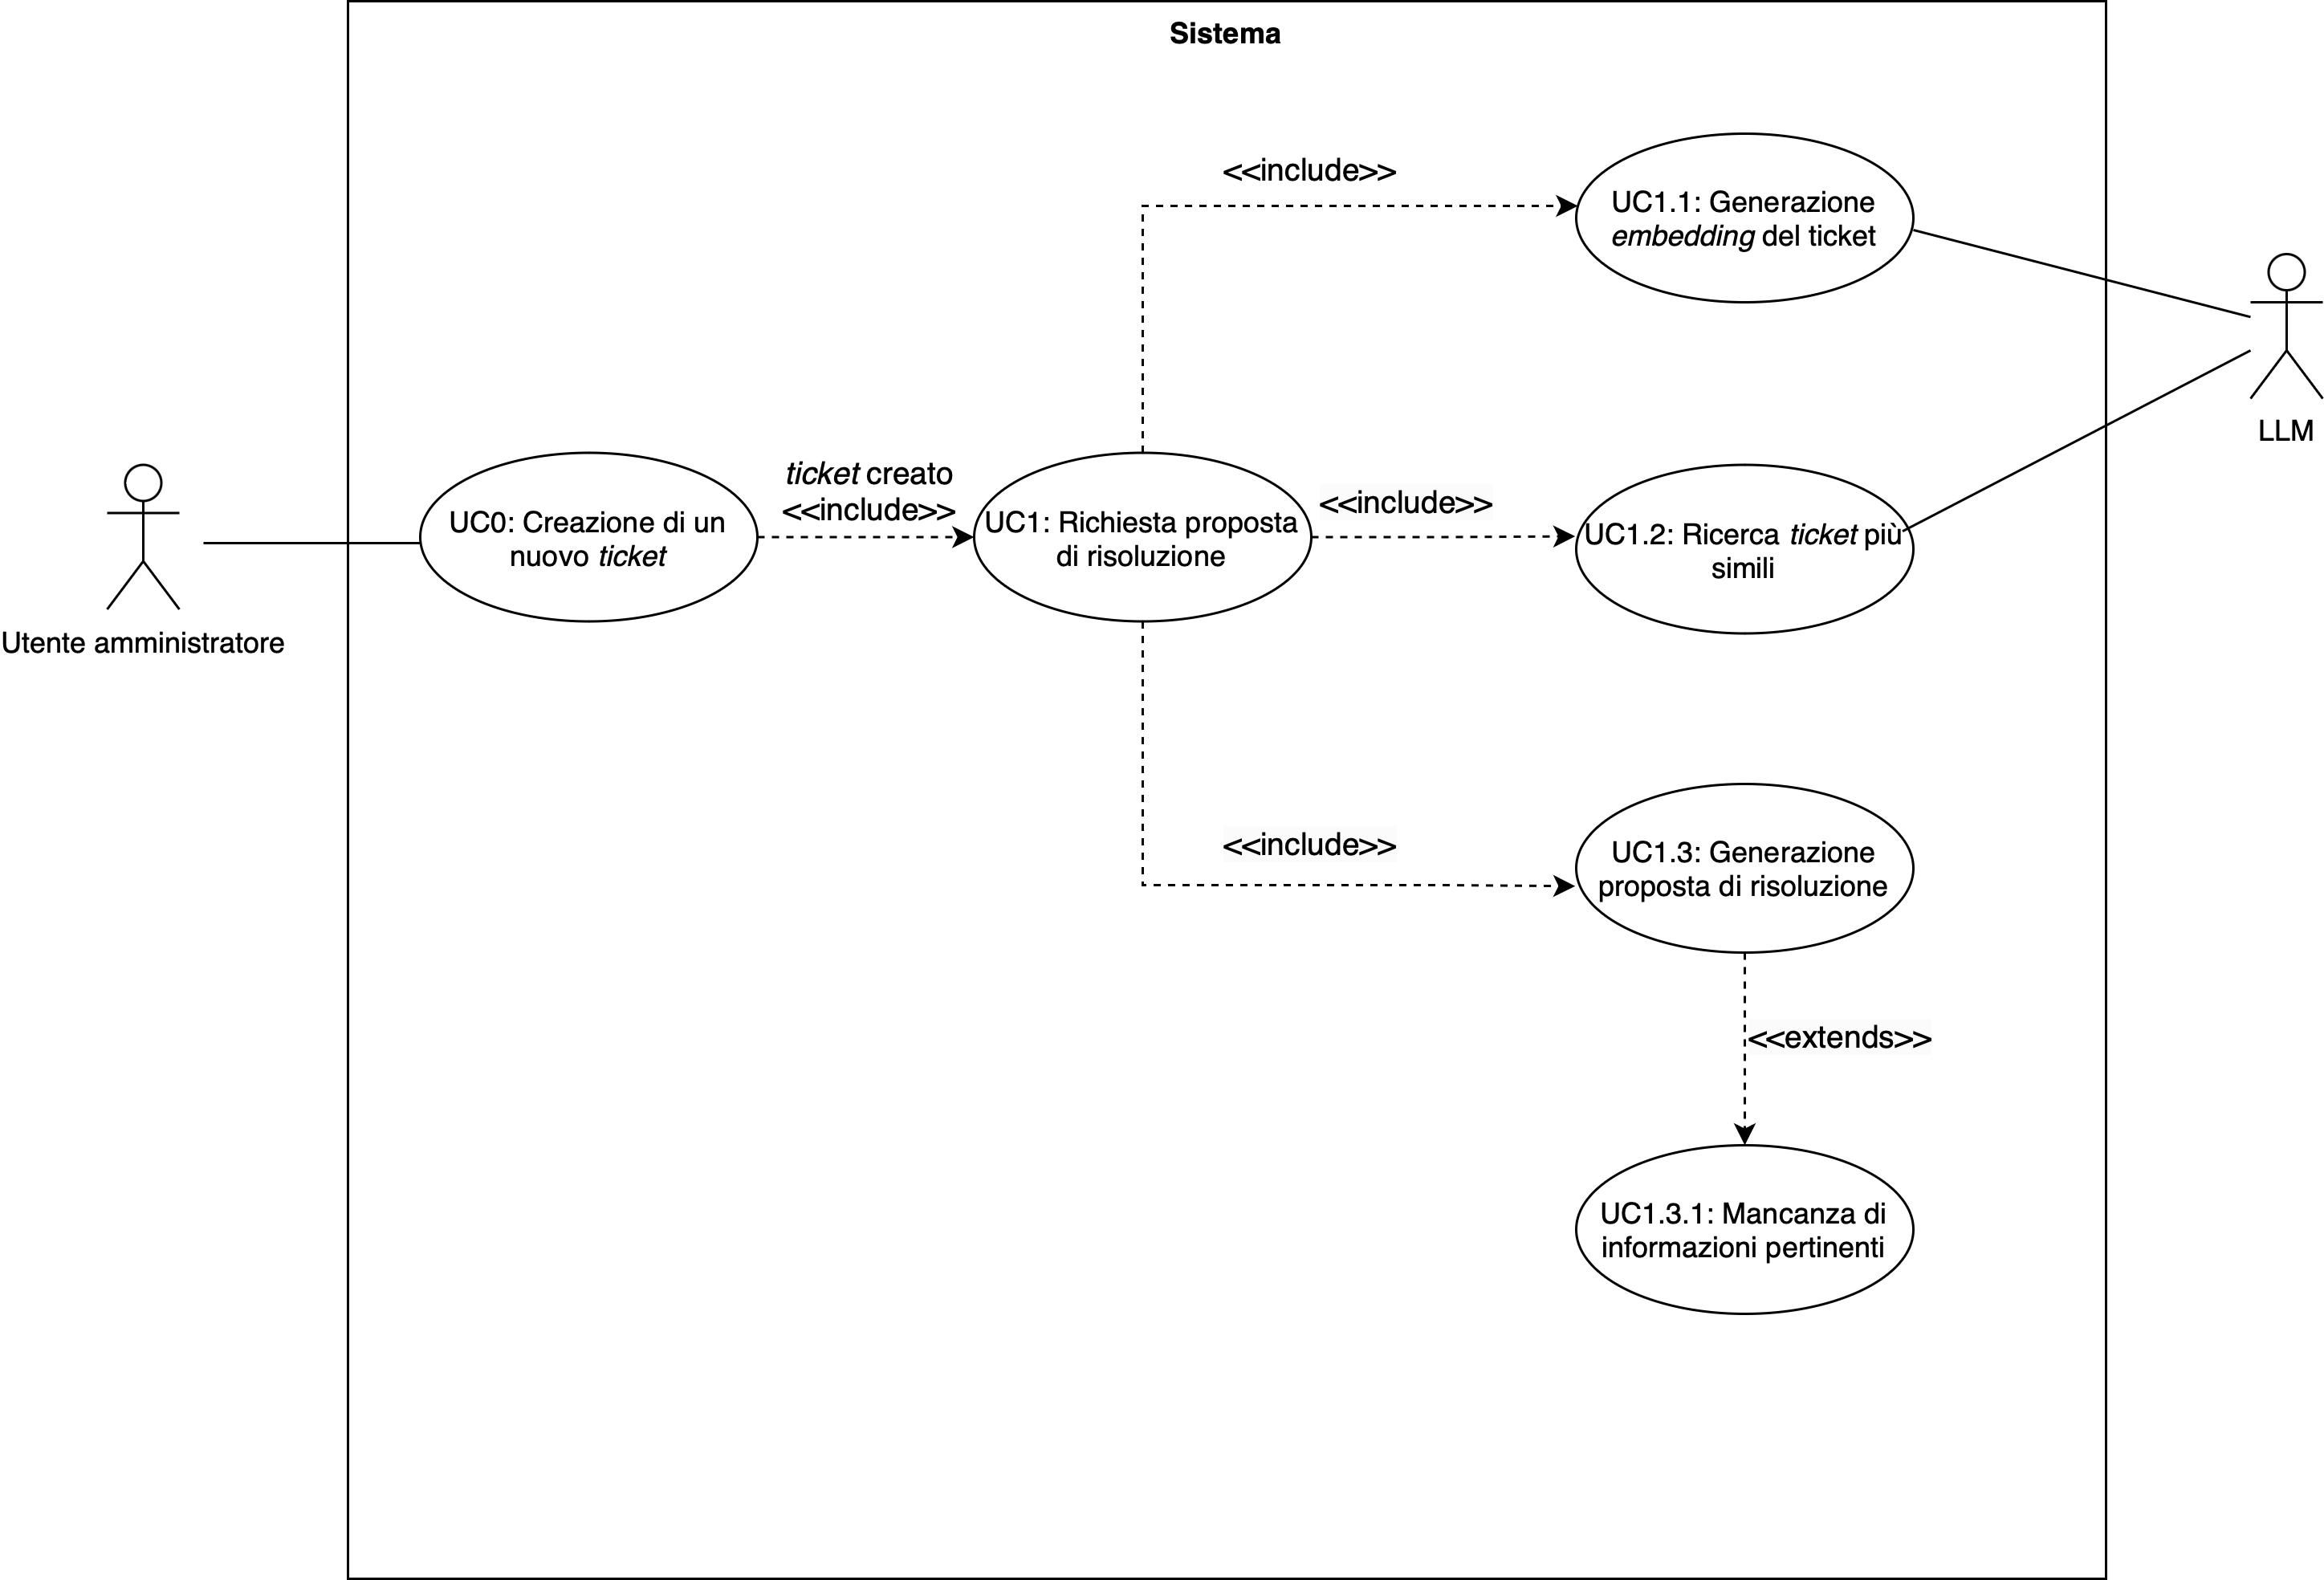
\includegraphics[width=0.8\textwidth]{uc1.png}
    \caption{Diagramma del caso d'uso UC1 e dei relativi sottocasi}
    \label{fig:UC1}
\end{figure}

\subsubsection{UC2: Chiusura di un \textit{ticket}}
\textbf{Attori principali}: Utente amministratore \\
\textbf{Precondizioni}: Il \textit{ticket} è stato completato \\
\textbf{Descrizione}: L'utente amministratore chiude il \textit{ticket} mettondolo in \textit{Done}\\ 
\textbf{Postcondizioni}: Il \textit{ticket} è stato chiuso \\

\begin{figure}[H]
    \centering
    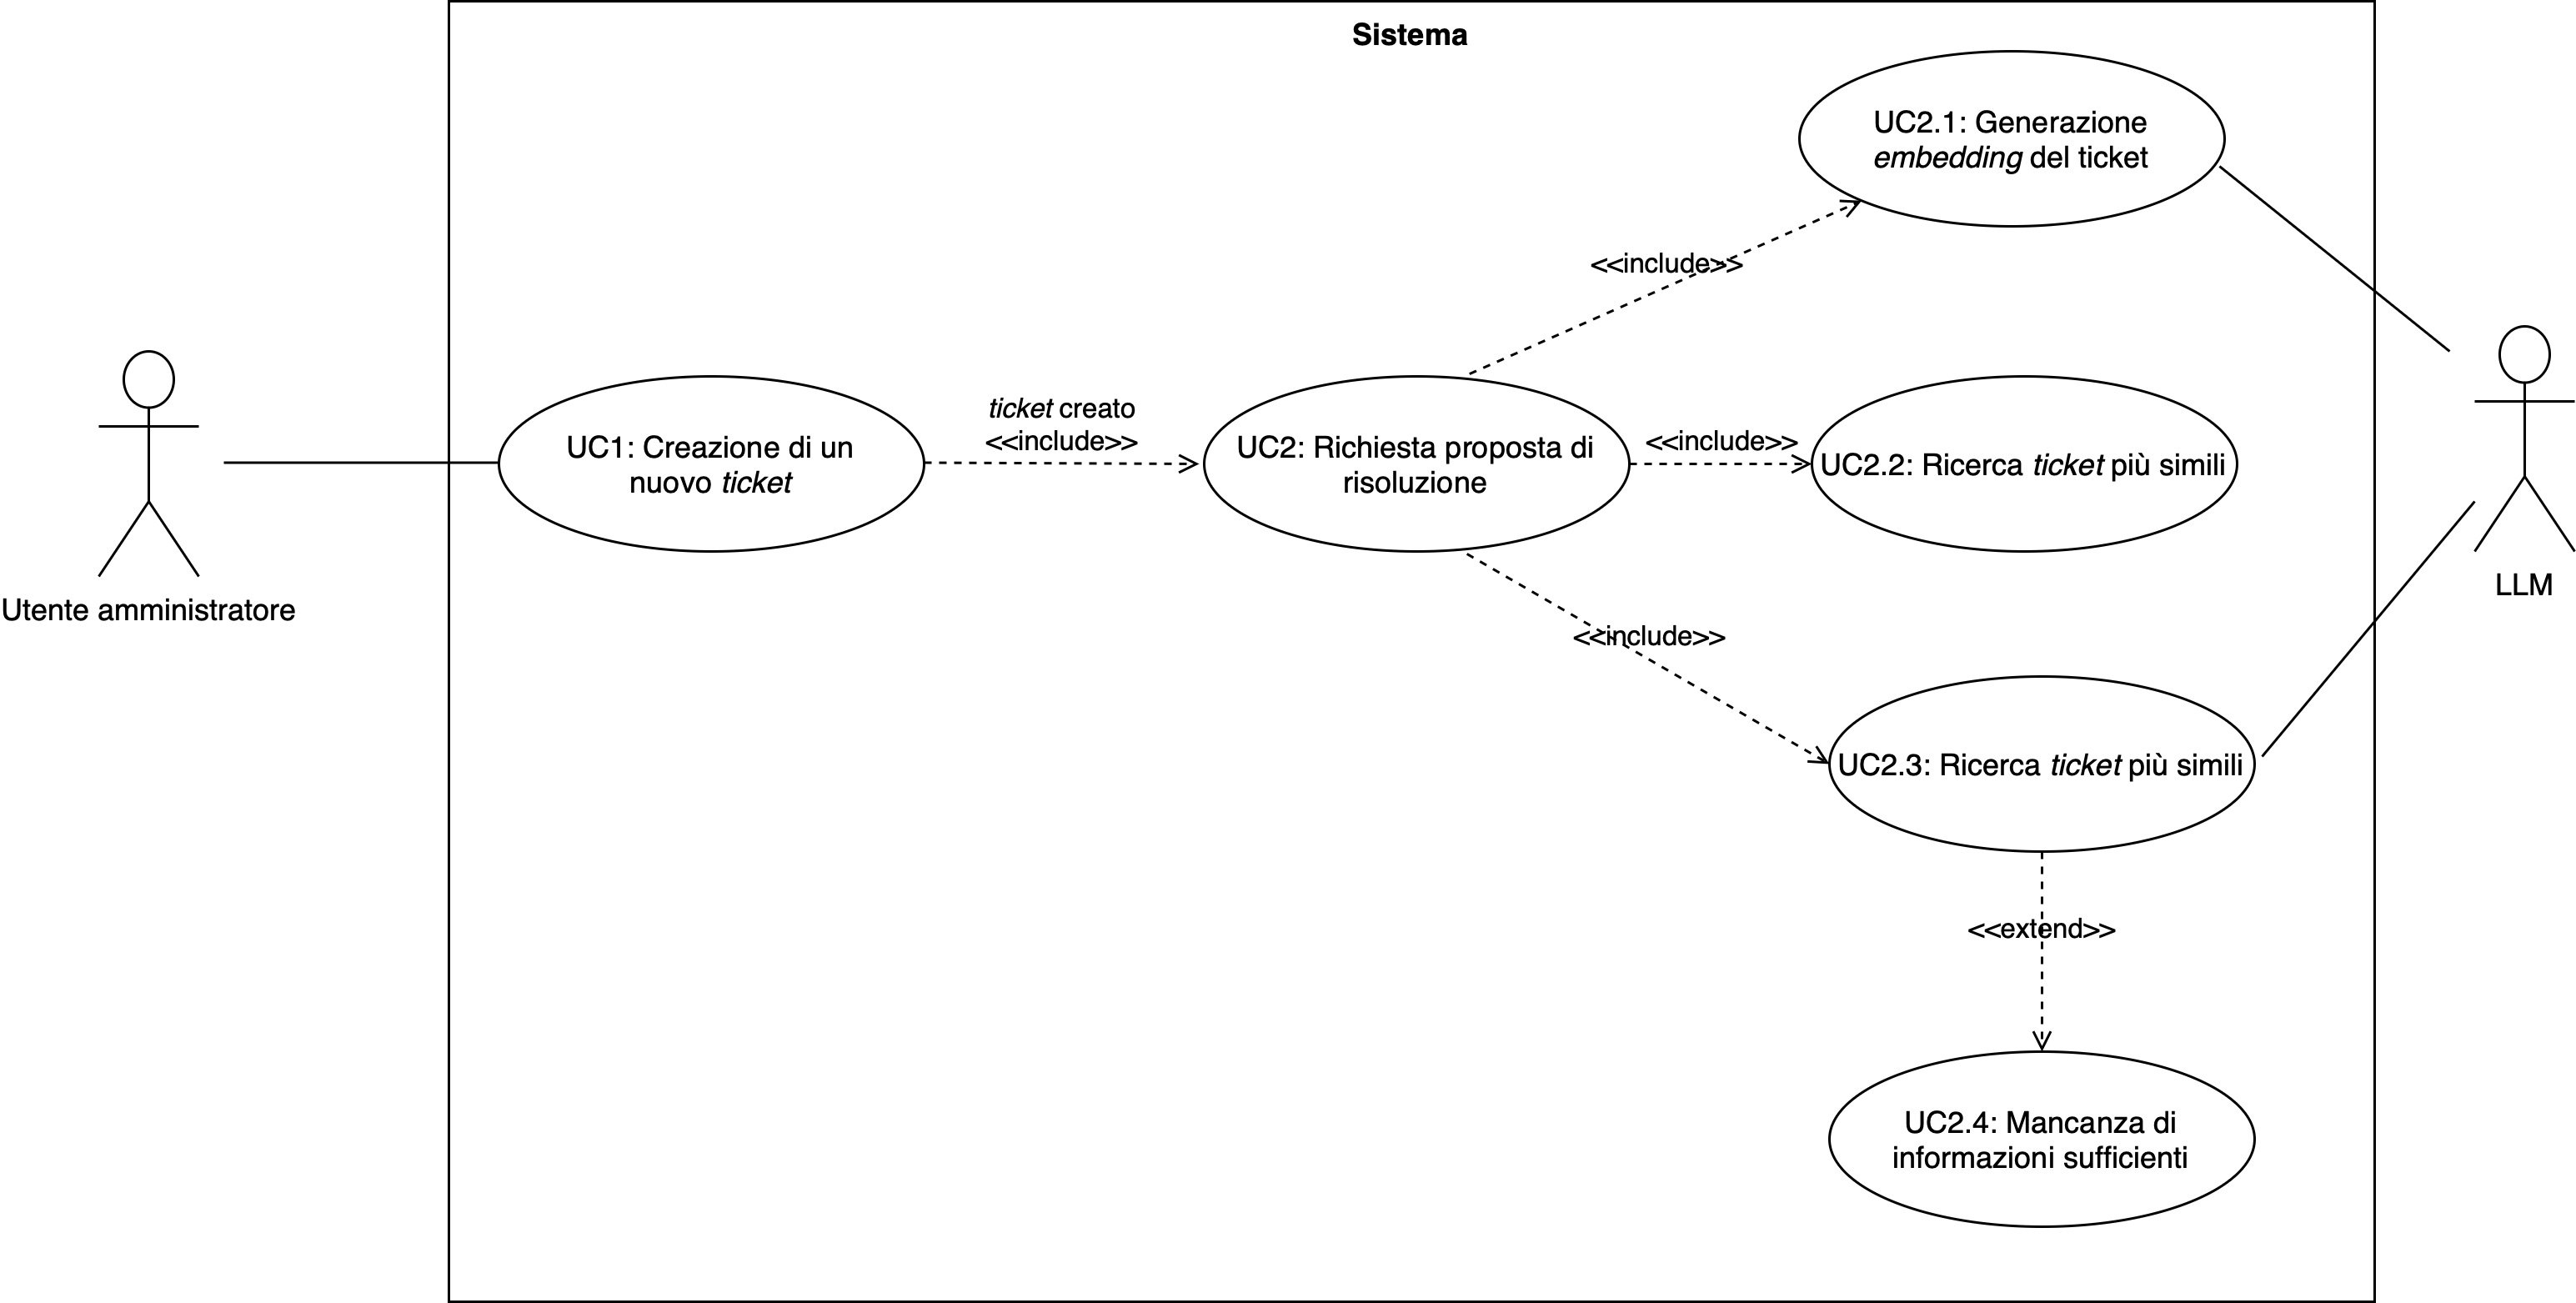
\includegraphics[width=0.55\textwidth]{uc2.png}
    \caption{Diagramma del caso d'uso UC2}
    \label{fig:UC2}
\end{figure}


\subsubsection{UC2.1: Generazione \gls{embedding-g} del \textit{ticket} completato}
\textbf{Attori principali}: \gls{llm} \\
\textbf{Precondizioni}: Il \textit{ticket} è stato chiuso \\
\textbf{Descrizione}: Viene richiesto all'\gls{llm} di generare l'\gls{embedding-g} del \textit{ticket} completato per poterlo poi salvare nel \textit{database} MongoDB \\
\textbf{Postcondizioni}: L'\gls{embedding-g} del \textit{ticket} è stato generato \\

\subsubsection{UC3: Salvataggio \textit{ticket} su \textit{database} MongoDB}
\textbf{Attori principali}: Sistema \\
\textbf{Precondizioni}: Il \textit{ticket} è stato compleato e in stato \textit{Done} \\
\textbf{Descrizione}: Il \textit{ticket} viene salvato su \textit{database} MongoDB con il suo relativo \textit{embedding} \\
\textbf{Postcondizioni}: Il \textit{ticket} è stato salvato su \textit{database} MongoDB con il suo relativo \textit{embedding} \\
\begin{figure}[H]
    \centering
    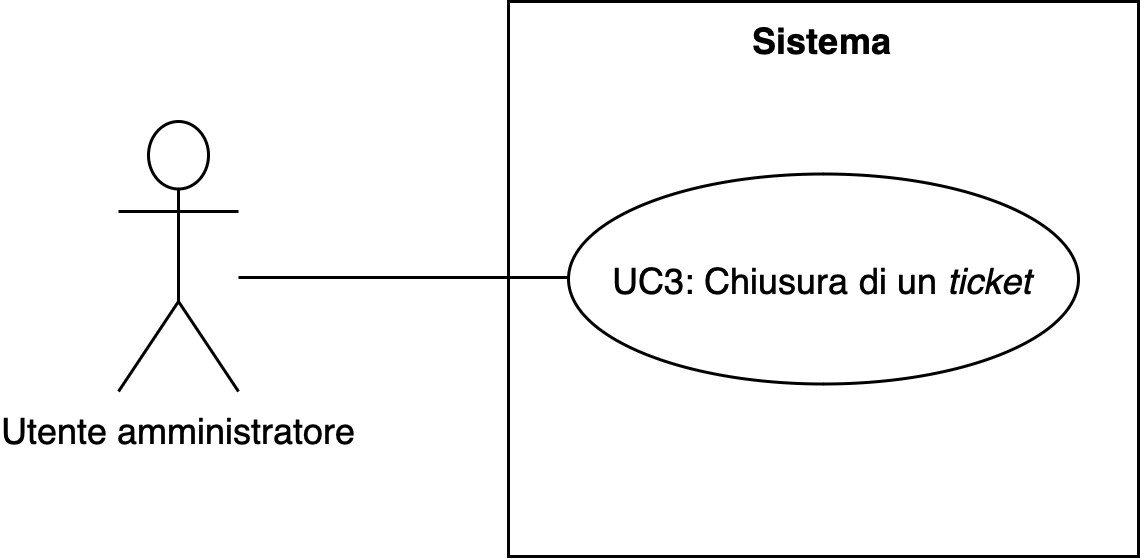
\includegraphics[width=0.78\textwidth]{uc3.png}
    \caption{Diagramma del caso d'uso UC3}
    \label{fig:UC5}
\end{figure}

\subsubsection{\textit{Chatbot}}

\subsubsection{UC0: Autenticazione nel \textit{chatbot}}
\textbf{Attori principali}: Utente generico \\
\textbf{Precondizioni}: L'utente vuole accedere al \textit{chatbot} \\
\textbf{Descrizione}: All'accesso al \textit{chatbot}, viene aperta una schermata di \textit{login} per l'autenticazione dell'utente \\
\textbf{Postcondizioni}: L'utente è autenticato nel \textit{chatbot} \\
\begin{figure}[H]
    \centering
    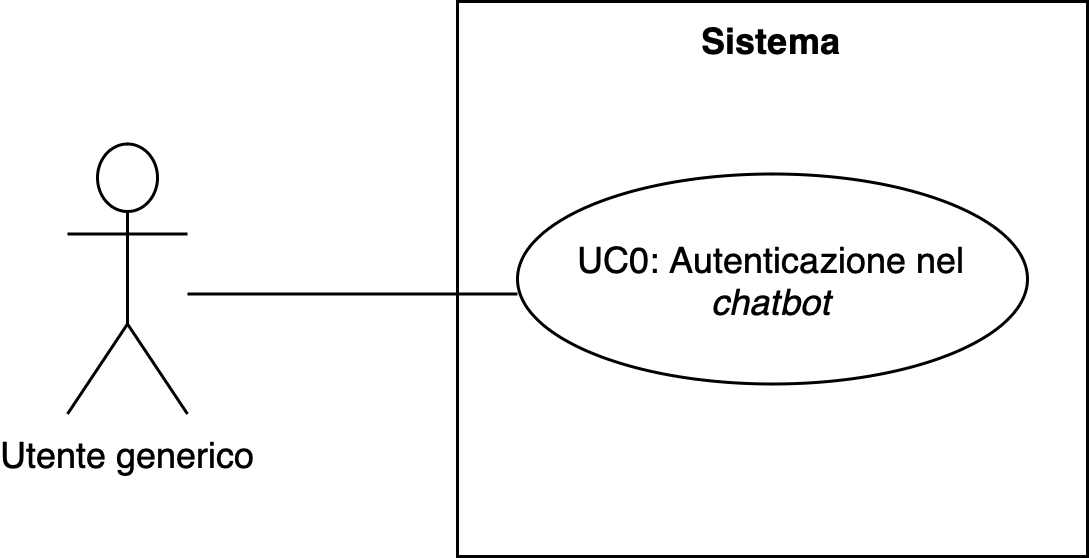
\includegraphics[width=0.53\textwidth]{uc0Chatbot.png}
    \caption{Diagramma del caso d'uso UC0 - \textit{Chatbot}}
    \label{fig:UC0Chatbot}
\end{figure}

\subsubsection{UC1: Autenticazione per il \textit{database} MongoDB}
\textbf{Attori principali}: Utente amministratore \\
\textbf{Precondizioni}: L'utente amministratore è autenticato nel \textit{chatbot} \\
\textbf{Descrizione}: L'utente amministratore si autentica per poter accedere al \textit{database} MongoDB e poter ricercare i \textit{ticket} più simili \\
\textbf{Postcondizioni}: L'utente amministratore è autenticato per il \textit{database} MongoDB \\
\begin{figure}[H]
    \centering
    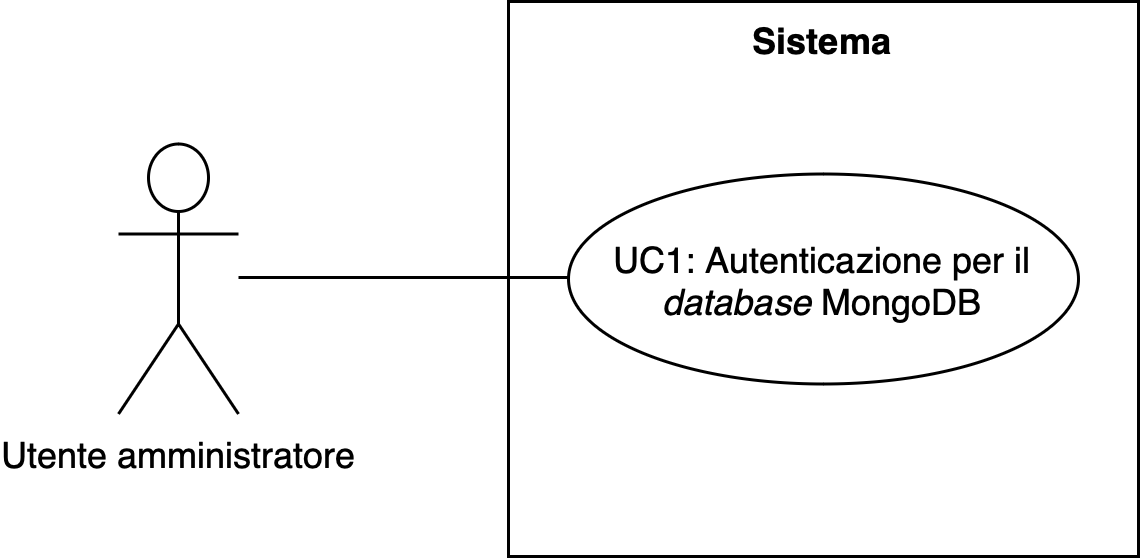
\includegraphics[width=0.53\textwidth]{uc1Chatbot.png}
    \caption{Diagramma del caso d'uso UC1 - \textit{Chatbot}}
    \label{fig:UC1Chatbot}
\end{figure}


\subsubsection{UC2: Scelta del modello \gls{llm}}
\textbf{Attori principali}: Utente amministratore \\
\textbf{Precondizioni}: L'utente amministratore è autenticato nel \textit{chatbot} \\
\textbf{Descrizione}: L'utente amministratore sceglie il modello \gls{llm} con cui interrogare il \textit{chatbot} \\
\textbf{Postcondizioni}: Il modello \gls{llm} è stato scelto \\
\begin{figure}[H]
    \centering
    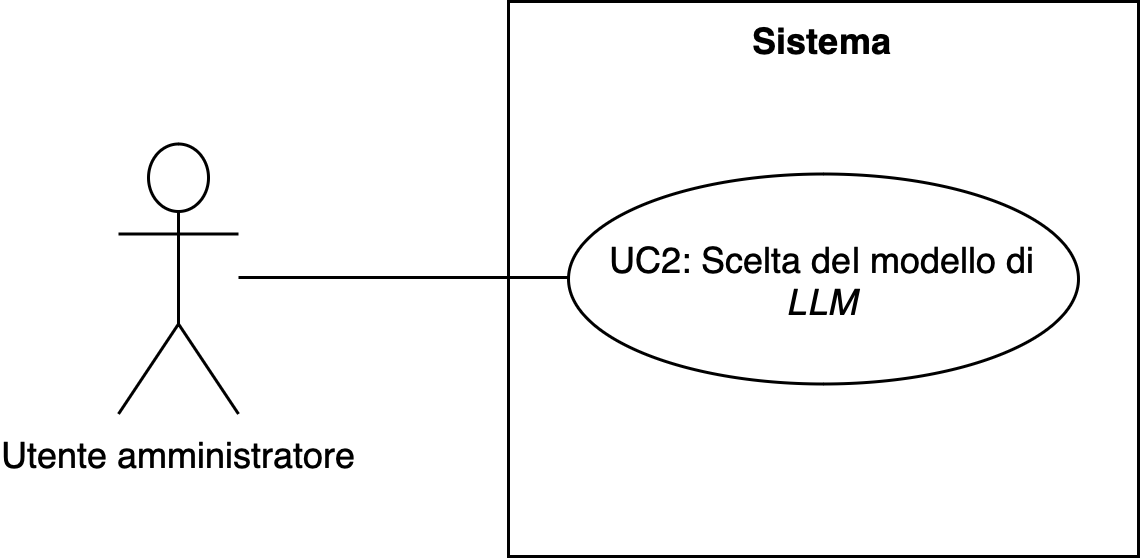
\includegraphics[width=0.55\textwidth]{uc2Chatbot.png}
    \caption{Diagramma del caso d'uso UC2 - \textit{Chatbot}}
    \label{fig:UC2Chatbot}
\end{figure}


\subsubsection{UC3: Inserimento del testo di un \textit{ticket} all'interno della \textit{chat} del \textit{chatbot}}
\textbf{Attori principali}: Utente amministratore \\
\textbf{Precondizioni}: L'utente amministratore ha scelto il modello \gls{llm} con cui interrogare il \textit{chatbot} \\
\textbf{Descrizione}: L'utente amministratore interroga il \textit{chatbot} sui \textit{ticket} Jira \\
\textbf{Postcondizioni}: Il \textit{chatbot} richiede la richiesta di proposta di risoluzione al sistema \\

\subsubsection{UC3.1: Generazione \gls{embedding-g} del testo inserito dall'utente}
\textbf{Attori principali}: \gls{llm} \\
\textbf{Precondizioni}: L'utente amministratore ha inserito il testo del \textit{ticket} per interrogare il \textit{chatbot} \\
\textbf{Descrizione}: Viene generato l'\gls{embedding-g} del testo inserito dall'utente per effettuare la ricerca dei \textit{ticket} completati più simili \\

\subsubsection{U3.2: Ricerca \textit{ticket} più simili all'interno del \textit{database} MongoDB}
\textbf{Attori principali}: Sistema \\
\textbf{Precondizioni}: È stato generato l'\gls{embedding-g} del testo inserito dall'utente \\
\textbf{Descrizione}: Il sistema effettua una ricerca vettoriale all'interno del \textit{database} con l'utilizzo dell'\gls{embedding-g}, per trovare i \textit{ticket} completati più simili al testo inserito dall'utente \\
\textbf{Postcondizioni}: I \textit{ticket} completati più simili vengono restuiti dal sistema \\

\subsubsection{UC3.3: Generazione proposta di risoluzione}
\textbf{Attori principali}: \gls{llm} \\
\textbf{Precondizioni}: Sono stati restituiti i \textit{ticket} completati più simili al testo inserito dall'utente \\
\textbf{Descrizione}: Viene richiesto all'\gls{llm} di generare una proposta di risoluzione per il testo inserito dall'utente usando come contesto i \textit{ticket} completati più simili \\
\textbf{Postcondizioni}: La proposta di risoluzione è stata generata e restituita all'utente, nell'interfaccia del \textit{chatbot} \\


\begin{figure}[H]
    \centering
    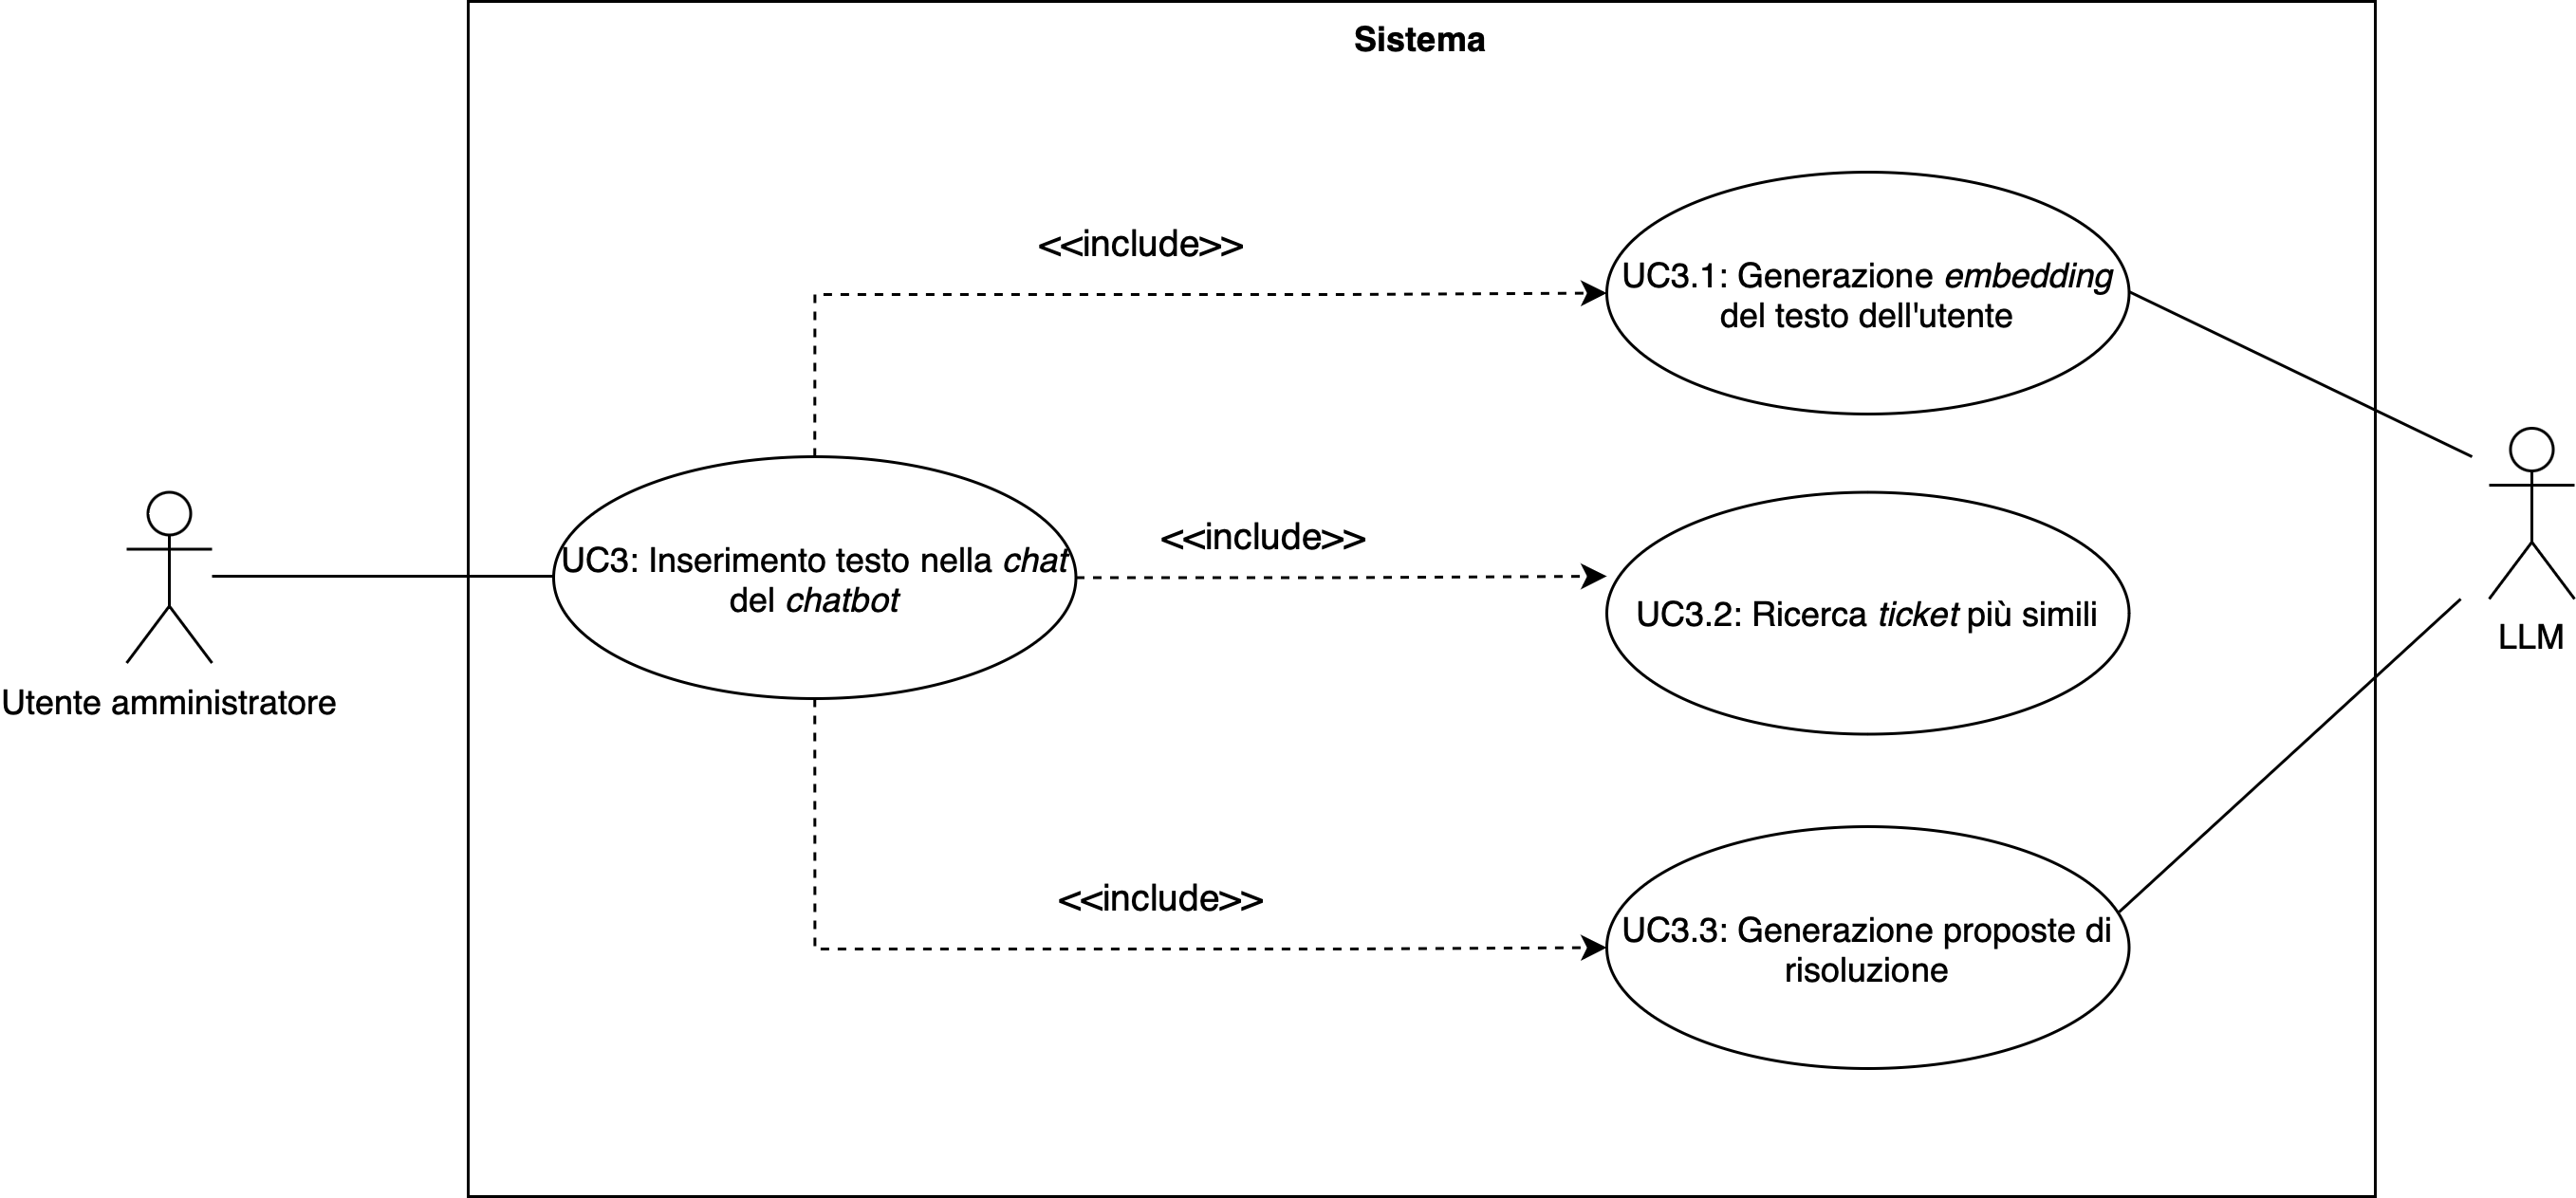
\includegraphics[width=0.86\textwidth]{uc3Chatbot.png}
    \caption{Diagramma del caso d'uso UC3 e dei relativi sottocasi - \textit{Chatbot}}
    \label{fig:UC3Chatbot}
\end{figure}

\subsection{Tracciamento dei requisiti}
Ho tracciato i requisiti individuati dai casi d'uso con la seguente notazione:
\begin{center}
    \textbf{R-[Tipologia][Importanza]-[Numero]}
\end{center}
dove: 
\begin{itemize}
    \item \textbf{R}: abbreviazione di Requisito
    \item \textbf{Tipologia}: Natura del requisito: \begin{itemize}
        \item \textbf{F}: Funzionale
        \item \textbf{V}: Vincolo
    \end{itemize}
    \item \textbf{Importanza}: Valore alfabetico che indica l'importanza del requisito: \begin{itemize}
        \item \textbf{O}: Obbligatorio
        \item \textbf{D}: Desiderabile
        \item \textbf{O}: Opzionale
    \end{itemize}
    \item \textbf{Numero}: Numero intero positivo progressivo del requisito
\end{itemize}

\renewcommand{\arraystretch}{1.4}
\begin{longtable}{|p{1.5cm}|p{5.5cm}|p{2cm}|p{2.5cm}|} 
    \hline
    \rowcolor{tableheader}\textbf{Codice} & \textbf{Descrizione} & \textbf{Importanza} & \textbf{Fonte}\\
    \hline
    \endfirsthead

    \rowcolor{tableheader}\textbf{Codice} & \textbf{Descrizione} & \textbf{Importanza} & \textbf{Fonte} \\
    \hline
    \endhead

    \hline
    \endfoot

    \hline
    \endlastfoot
    \hline
    R-FO-1 & Il sistema deve eseguire una richiesta di generazione di proposta di risoluzione quando un \textit{ticket} viene creato & Obbligatorio & UC1 (Jira) \\
    \hline
    \rowcolor{tableevenrow} R-FO-2 & Il sistema deve poter interrogare un \gls{llm} per la creazione dell'\gls{embedding-g} del \textit{ticket} creato & Obbligatorio & UC1.1 (Jira) \\
    \hline
    R-FO-3 & Il sistema deve effettuare una ricerca dei ticket completati più simili al \textit{ticket} creato, nel \textit{database} & Obbligatorio & UC1.2 (Jira) \\
    \hline
    \rowcolor{tableevenrow} R-FO-4 & Il sistema deve poter interrogare un \gls{llm} per generare una proposta di risoluzione utilizzando come contesto i \textit{ticket} completati più simili. & Obbligatorio & UC1.3 (Jira) \\
    \hline
    R-FO-5 & Il sistema deve poter interrogare un \gls{llm} per generare una risposta standard in caso di mancanza di \textit{ticket} completati simili. & Obbligatorio & UC1.4 (Jira) \\
    \hline
    \rowcolor{tableevenrow} R-FO-6 & Il sistema deve poter interrogare un \gls{llm} per la generazione dell'\gls{embedding-g} del \textit{ticket} completato per salvarlo nel \textit{database} & Obbligatorio & UC2.1 (Jira) \\
    \hline
    R-FO-7 & Il sistema deve permettere il salvataggio del \textit{ticket} completato e del relativo \gls{embedding-g} nel \textit{database}. & Obbligatorio & UC3 (Jira) \\
    \hline
    \rowcolor{tableevenrow} R-FO-8 & Il sistema deve permettere l'autenticazione dell'utente nel \textit{chatbot}. & Obbligatorio & UC0 (Chatbot) \\
    \hline
    R-FO-9 & Il sistema deve permettere l'autenticazione dell'utente amministratore per accedere al \textit{database}. & Obbligatorio & UC1 (Chatbot) \\
    \hline
    \rowcolor{tableevenrow} R-FO-10 & Il sistema deve permettere la scelta del modello \gls{llm} con cui interrogare il \textit{chatbot}. & Obbligatorio & UC2 (Chatbot) \\
    \hline
    R-FO-11 & Il sistema deve permettere l'interrogazione al modello \gls{llm} tramite una \textit{chat}. & Obbligatorio & UC3 (Chatbot) \\
    \hline
    \rowcolor{tableevenrow} R-FO-12 & Il sistema deve poter interrogare un \gls{llm} per generare l'\gls{embedding-g} del testo inserito dall'utente. & Obbligatorio & UC3.1 (Chatbot) \\
    \hline
    R-FO-13 & Il sistema deve permettere la ricerca dei ticket più simili all'interno del \textit{database}. & Obbligatorio & UC3.2 (Chatbot) \\
    \hline
    \rowcolor{tableevenrow} R-FO-14 & Il sistema deve poter interrogare un \gls{llm} per la generazione di una proposta di risoluzione basata sui \textit{ticket} simili. & Obbligatorio & UC3.3 (Chatbot) \\
    \hline
    R-VO-15 & Il sistema Jira deve essere sviluppato utilizzando il Serverless \textit{framework}  & Obbligatorio & Interna \\
    \hline
    \rowcolor{tableevenrow} R-VO-16 & Il \textit{database} utilizzato deve essere MongoDB & Obbligatorio & Interna \\
    \hline
    R-VO-17 & Il \textit{chatbot} deve essere sviluppato utilizzando il \textit{framework} Streamlit & Obbligatorio & Interna \\
    \hline
    \rowcolor{tableevenrow} R-VO-18 & L'autenticazione nel \textit{chatbot} deve utilizzare il servizio \gls{aws} Cognito & Obbligatorio & Interna \\

    
    \hline
    \caption{Tracciamento dei requisiti}
    \label{tab:tracciamentoRequisiti}
\end{longtable}

\section{Progettazione}
\subsection{RAG e selezione del modello LLM} \label{sec:rag}
L'integrazione e l'utilizzo di \gls{llm} e \gls{rag} rappresenta il fulcro dei progetti che ho sviluppato durante lo \textit{stage}.
Di seguito descrivo il funzionamento della \gls{rag} e mostro che modello ho selezionato per la generazione di testo. Mostrerò anche il \textit{benchmark} creato con il quale ho selezionato il modello migliore per la generazione di testo.
\subsubsection{Funzionamento della RAG}
Il funzionamento della \gls{rag} può essere diviso in più fasi, qui di seguito elencate:
\begin{itemize}
    \item \textbf{Reperimento di dati di addestramento}: per prima cosa è necessario reperire dei dati da fonti esterne o produrli autonomamente in modo da arrichire la conoscenza del modello. Nel progetto di \textit{stage} i dati sono stati prodotti autonomamente, risultato delle attività svolte durante la 2° settimana come mostrato nella tabella \ref{tab:prevAttività};
    \item \textbf{Salvataggio dei dati in un \textit{database} vettoriale}: i dati prodotti vengono salvati all'interno di un \textit{database} vettoriale con il loro \gls{embedding-g} associato. Questo processo facilita il recupero delle informazioni rilevanti per la generazione di testo. Nel progetti di \textit{stage} i dati sono stati salvati all'interno di un \textit{database} MongoDB;
    \item \textbf{Recupero delle informazioni pertinenti}: quando l'utente crea una \textit{query}, il sistema utilizza il \textit{database} vettoriale per recuperare le informazioni e i dati più pertinenti alla richiesta dell'utente. La ricerca coinvolge l'uso di tecniche di \gls{knn} per ricercare i vettori più simili al vettore della \textit{query}. Tramite questa ricerca si ottengono i dati più pertinenti alla richiesta dell'utente. Nel progetto di \textit{stage} il \textit{database} MongoDB permetteva la creazione di un indice vettoriale adibito alla ricerca vettoriale. Nella creazione dell'indice si poteva specificare il numero di dimensione del vettore, e la funzione di similarità combinata con il \gls{knn-g} utilizzata per la ricerca;
    \begin{figure}[H]
        \centering  
        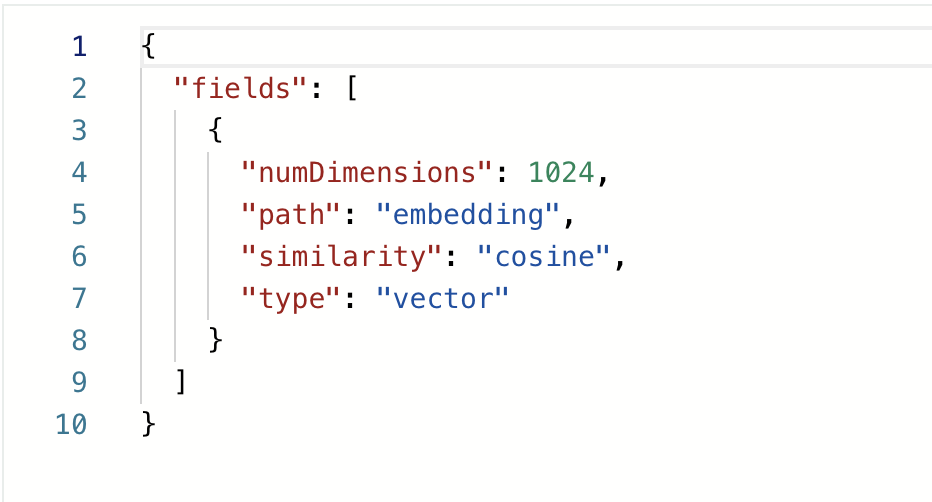
\includegraphics[width=0.65\textwidth]{indexMongoDB.png}
        \caption{Indice vettoriale creato su MongoDB}
        \label{fig:indexMongoDB}
    \end{figure}
    \item \textbf{Generazione della risposta}: le informazioni più pertinenti vengono combinate con la \textit{query} data inizialmente dall'utente per creare un \textit{prompt} che verrà inviato al \gls{llm} che generà la risposta utilizzando il contesto fornito.
\end{itemize}

\subsubsection{\textit{Prompt engineering}}
Come aspetto cruciale per la generazione di proposte di risoluzione di qualità, ho dovuto creare un \textit{prompt} che permettesse al modello di generare proposte di risoluzioni corrette utilizzando il contesto fornito. Inizialmente per testare la qualità del \textit{prompt} creato, ho utilizzato il modello \textit{MistralLarge} di \gls{aws} Bedrock tramite la \textit{console}. La scelta è ricaduta su questo modello in quanto si è dimostrato il più performante tra quelli offerti.
La creazione del \textit{prompt} è stata effettuata ispirandosi alle pratiche del \gls{promptenginnering-g}, ovvero un processo di progettazione e ottimizzazione di \textit{prompt}. L'approccio che ho utilizzato è stato fondamentale un \textit{trial and error} ed è consistito nel testare gli svariati \textit{prompt} creati con il modello \textit{MistralLarge} per valutare la qualità delle proposte di risoluzione generate.
Di seguito mostro il prompt finale creato per il sistema di proposte di risoluzione Jira:
\begin{Verbatim}[frame=single, fontsize=\small]
    Ti fornisco le seguenti informazioni estratte dai documenti:
    ${JSON.stringify(results)}.
    La domanda posta è: "${queryText}".
    
    Istruzioni per la risposta:
    1. Rispondi ESCLUSIVAMENTE in base alle informazioni contenute nei 
       documenti forniti.
    2. NON aggiungere interpretazioni, opinioni o ragionamenti personali.
    3. Se i documenti trattano problemi simili, fornisci TUTTE le possibili 
       soluzioni basate sulle risoluzioni presenti.
    4. Descrivi in modo chiaro ed esaustivo OGNI soluzione possibile, 
       senza limitarti a una sola opzione.
    5. Se le informazioni necessarie non sono presenti nei documenti e i 
       problemi non sono simili, dichiara ESPLICITAMENTE l'impossibilità di 
       rispondere.
    6. La risposta deve essere in lingua italiana.
    7. Inizia SEMPRE la risposta con "In base ai precedenti ticket:".
    8. Includi link nel formato:
       https://${process.env.JIRA_DOMAIN}/jira/servicedesk/projects/
       ${process.env.JIRA_PROJECT_KEY}/queues/custom/66/${key}
    9. Utilizza il seguente formato per ogni soluzione, se disponibile:
        -[Chiave del ticket][Descrizione dettagliata della risoluzione][Link]
    
    10. Se non è possibile fornire una risposta, specificalo 
        chiaramente SENZA aggiungere ulteriori informazioni o speculazioni.
    
    Attieniti RIGOROSAMENTE a queste istruzioni senza deviazioni.
\end{Verbatim}
\noindent
Per quanto riguarda la creazione del \textit{prompt} per il \textit{chatbot}, ho seguito lo stesso approccio, ma con delle modifiche per adattarlo al contesto del \textit{chatbot}. Di seguito mostro il prompt finale creato per il \textit{chatbot}:
\begin{Verbatim}[frame=single, fontsize=\small]
    Sei un assistente specializzato che fornisce informazioni e soluzioni 
    basandosi esclusivamente sul database e sui documenti di supporto 
    disponibili.  Il tuo compito è analizzare le domande degli 
    utenti e rispondere in modo appropriato seguendo 
    queste linee guida:

    1. Formato della domanda:
    - Verifica che la domanda dell'utente sia nel formato corretto: 
    [Domanda, codice della componente]
    - Se manca il codice alfanumerico della componente, rispondi solo che
     non puoi procedere senza queste informazioni e richiedi i dettagli 
     nel formato corretto
    - Non fornire soluzioni o informazioni dai documenti se il formato 
    non è corretto

    2. Analisi dei documenti:
    - Se il formato è corretto, cerca nei documenti componenti uguali o 
    simili,
     anche se non trattano esattamente lo stesso problema
    - Verifica attentamente la pertinenza delle informazioni trovate

    3. Formulazione della risposta:
    - Basa la tua risposta rigorosamente sulle informazioni presenti nei 
    documenti, senza aggiungere interpretazioni o ragionamenti personali
    - La risposta deve essere in italiano, esaustiva e descrittiva
    - Inizia sempre con "In base ai precedenti ticket:"
    - Se pertinente, includi:
        • Riassunto della descrizione del ticket
        • Codice della componente
        • Soluzione proposta
        • Chiave del ticket
    - Non utilizzare formattazione, bullet points o elenchi
    - Termina la risposta dopo aver suggerito una soluzione o dichiarato 
    l'impossibilità di rispondere
    - Non aggiungere spiegazioni o ragionamenti ulteriori
    - Evita spazi o caratteri speciali alla fine della risposta

    4. In caso di mancanza di informazioni:
    - Se non trovi informazioni pertinenti o componenti simili, dichiara 
    chiaramente che non puoi fornire una risposta alla domanda

    Context: {context}
    User question: {input_text}
    Ricorda: analizza attentamente il formato della domanda prima di 
    procedere con la ricerca nei documenti e la formulazione della 
    risposta.
\end{Verbatim}
\subsubsection{Selezione del modello \gls{llm}}
La selezione del modello rappresenta una scelta cruciale per una proposta di risoluzione coerente e di qualità. Come ho mostrato nella tabella \ref{tab:prevAttività} ho creato un \textit{benchmark} per selezionare quale tra i modelli più performanti offerti da \gls{aws} Bedrock fosse il migliore per il contesto dei due progetti.
Per la creazione del \textit{benchmark} ho creato una serie di \textit{ticket} fittizzi a cui ho associato delle proposte di risoluzione in base ai \textit{ticket} completati contenuti nel \textit{database}. In seguito, per ognuno di questi ticket veniva richiesta una proposta di risoluzione ai vari modelli da testare e le risposte venivano valutato da un ulteriore modello, di cui ho avuto modo di poterne testare l'accuratezza tramite la \textit{console} di \gls{aws} Bedrock.
\begin{figure}[H]
    \centering
    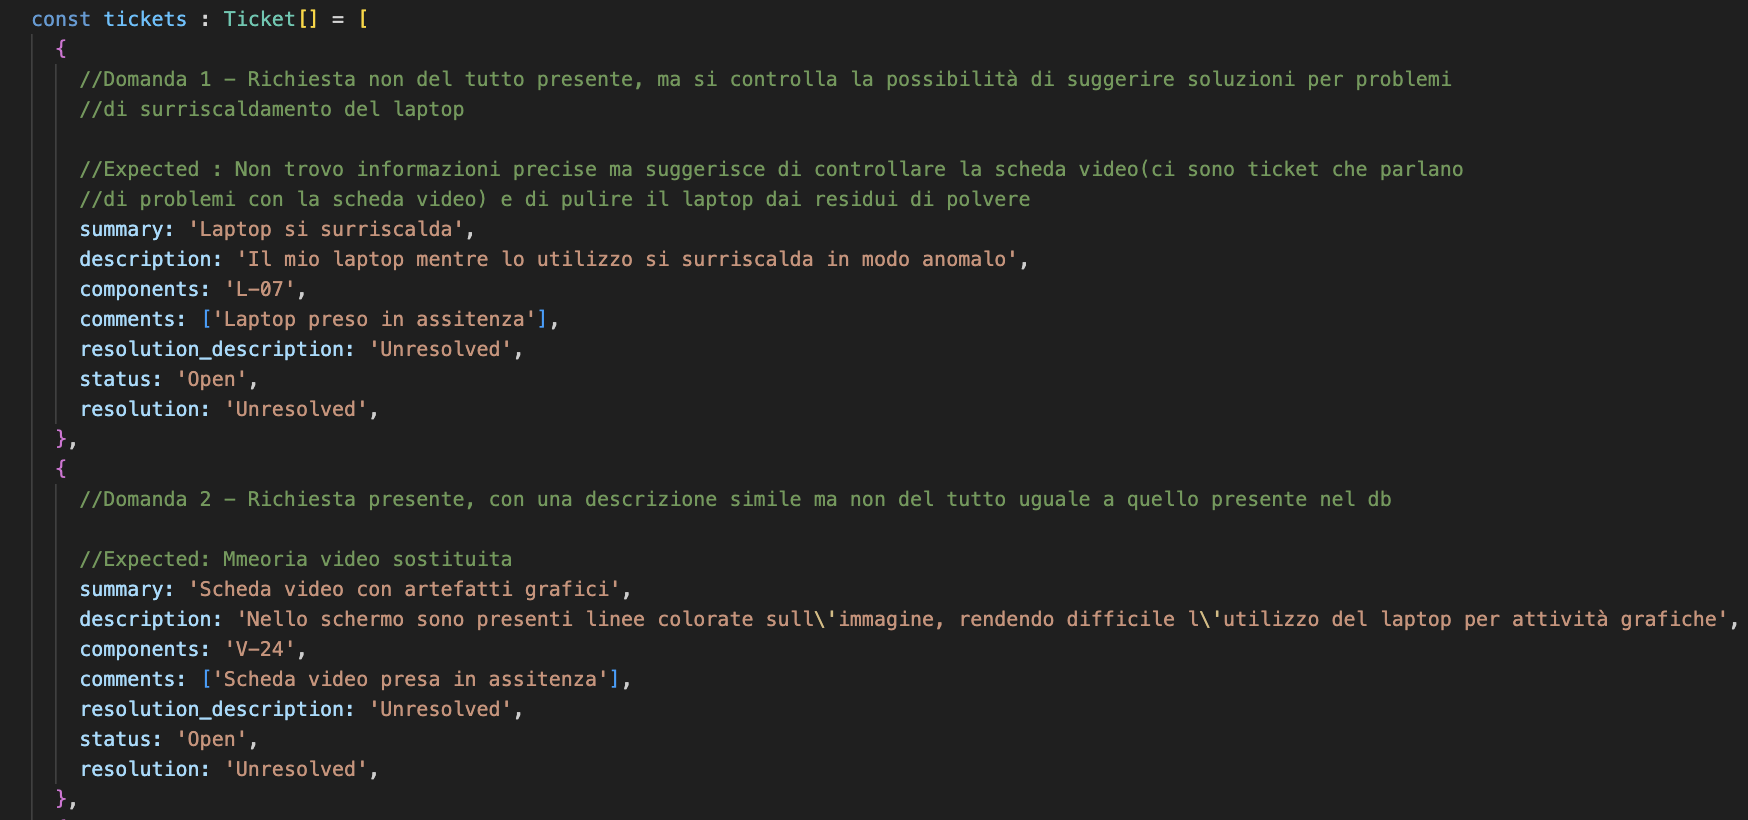
\includegraphics[width=0.85\textwidth]{ticketBenchmarkExample.png}
    \caption{Esempio \textit{ticket} fittizzi creati per il \textit{benchmark}}
    \label{fig:Ticketbenchmark}
\end{figure}
\noindent
Come mostro nell'immagine \ref{fig:Ticketbenchmark}, i \textit{ticket} creati possiedono tutti i dati che il sistema riceve quando un \textit{ticket} viene creato su Jira. Alcuni di questi dati sono lasciati con valori \textit{default} in quanto lo scopo era quello di valutare la qualità delle proposte di risoluzione dei vari modelli. 
Come sistema di \textit{scoring}, come ho accennato in precedenza, ho utilizzato il modello \textit{MistralLarge} di \gls{aws} Bedrock. Tramite l'utilizzo di questo modello ho potuto attribuire un punteggio di similarità tra la proposta di risoluzione generata dal modello e la proposta di risoluzione attesa in modo automatico. La scala di valutazione del punteggio di similarità varia tra 0 (risposte totalmente diverse) e 1 (risposte identiche). \\
In figura \ref{fig:benchmarkArchitecture} mostro l'architettura del \textit{benchmark}:
\begin{figure}[H]
    \centering
    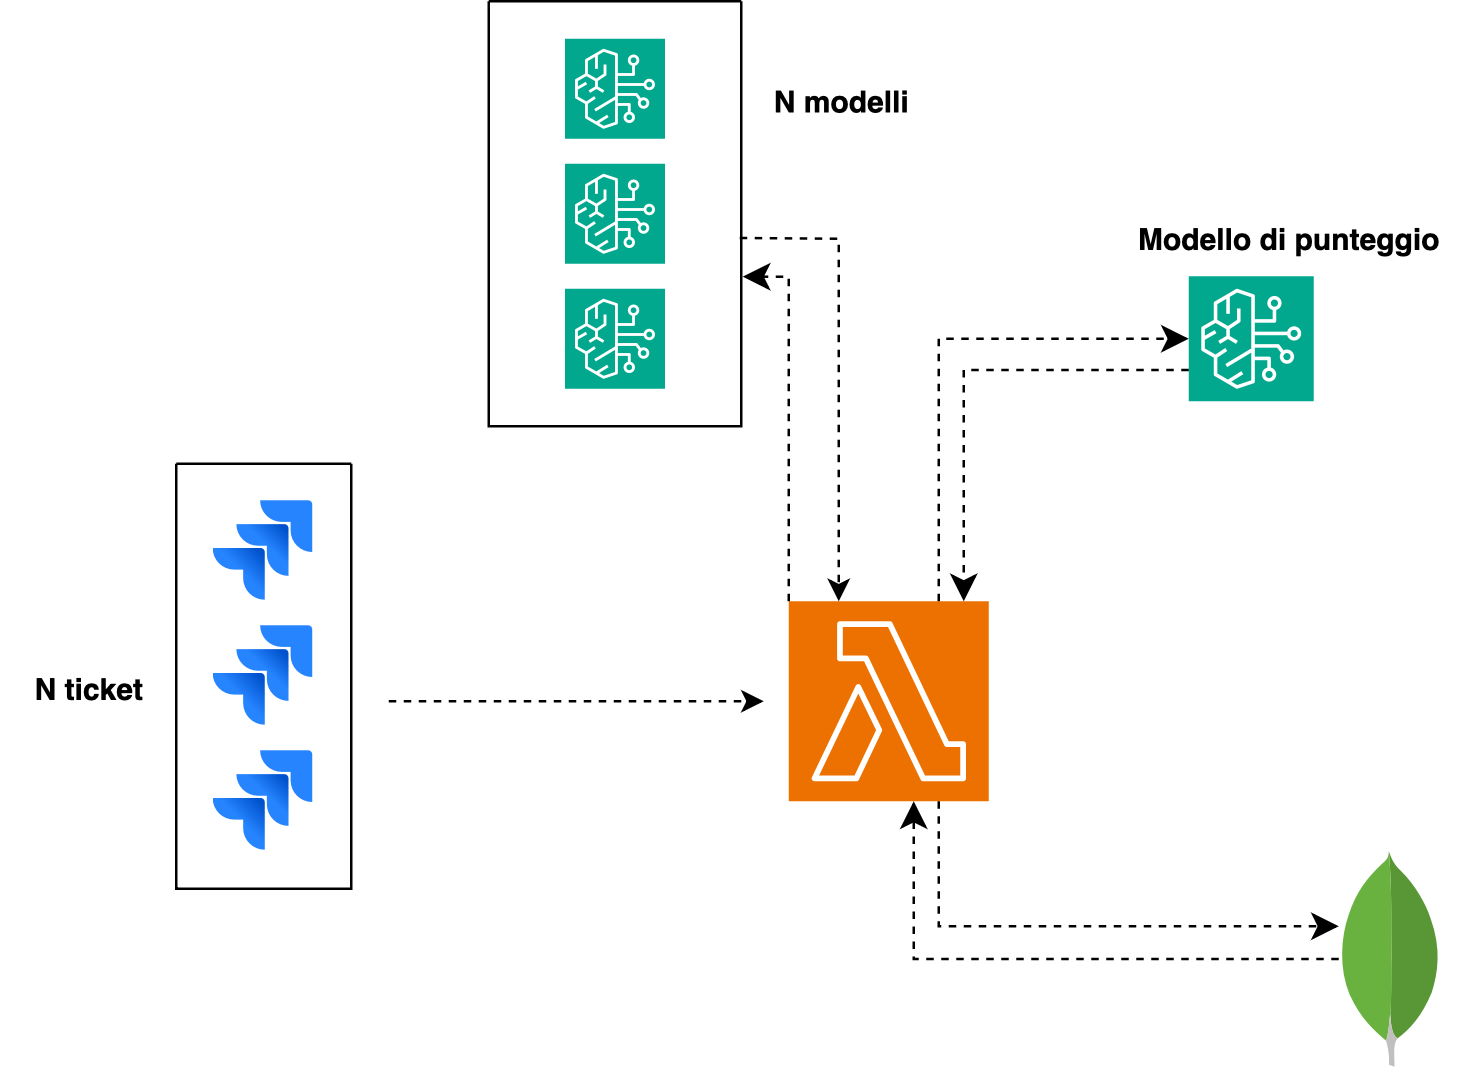
\includegraphics[width=0.9\textwidth]{architetturaBenchmark.png}
    \caption{Architettura del \textit{benchmark}}
    \label{fig:benchmarkArchitecture}
\noindent
Come mostro nell'immagine \ref{fig:benchmarkArchitecture}, il \textit{benchmark} è composto da tre componenti principali:
\begin{itemize}
    \item \textbf{N \textit{ticket} fittizzi}: insieme di \textit{ticket} creati per valutare la qualità delle proposte di risoluzione dei vari modelli, come mostrato nell'immagine \ref{fig:Ticketbenchmark};
    \item \textbf{N Modelli}: insieme di \gls{llm} offerti da \gls{aws} Bedrock che interrogo per generare proposte di risoluzione per gli N \textit{ticket} fittizzi e li restituisce alla funzione \textit{lambda}; 
    \item \textbf{\textit{Database}}: componente che tramite la ricerca vettoriale trova i \textit{ticket} completati più simili ai \textit{ticket} fittizzi creati. 
    \item \textbf{Modello di punteggio}: modello che valuta la qualità delle proposte di risoluzione generate dai vari modelli interrogati. Restituisce un numero intero positivo compreso tra 0 (risposta totalmente diversa) e 1 (risposta identica).
\end{itemize}
\end{figure}
In figura \ref{fig:benchmarkResult} mostro il risultato del \textit{benchmark}:
\begin{figure}[H]
    \centering
    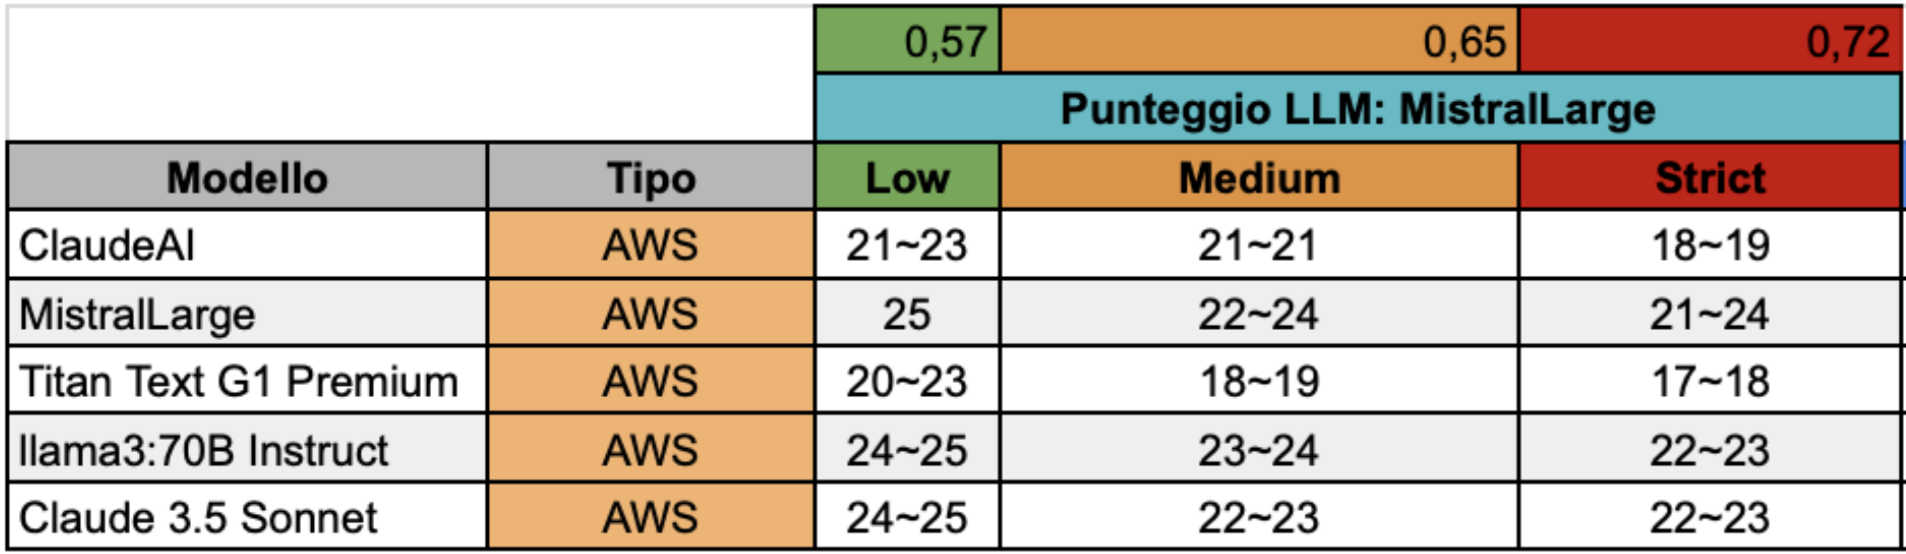
\includegraphics[width=0.8\textwidth]{benchmark.png}
    \caption{Risultato del \textit{benchmark}}
    \label{fig:benchmarkResult}
\end{figure}
\noindent
Il punteggio relativo ad ogni modello è suddiviso in tre categorie:
\begin{itemize}
    \item \textbf{Low}: punteggio di similarita maggiore di 0,57 incluso;
    \item \textbf{Medium}: punteggio di similarità maggiore di 0,65 incluso;
    \item \textbf{Strict}: punteggio di similarità maggiore di 0,72 incluso;
\end{itemize}
Il punteggio attribuito ai vari modelli però è un indicatore di qualità rispetto alle proposte di risoluzione attese da me create. Questo implica che modelli che hanno ottenuto un punteggio più basso generano comunque proposte di risoluzione corrette, ma non nel formato da me richiesto. Questo è un aspetto che ho dovuto considerare nella scelta del modello.
Come si può notare dall'immagine \ref{fig:benchmarkResult}, il modello \textit{Claude3.5 Sonnet} e \textit{MistralLarge} hanno ottenuto i migliori risultati. Tuttavia la scelta del modello è ricaduta su Claude3.5Sonnet in quanto ha dimostrato di generare proposte di risoluzione di qualità superiore rispetto a \textit{MistralLarge}.\\
Come modello per la generazione di \gls{embedding-g} invece la scelta è ricaduta su \textit{Titan Text Embeddings V2} in quanto rispetto alle alternative offerte da \gls{aws} Bedrock, permetteva di generare \gls{embedding-g} con una dimensione minore ma con qualità superiore rispetto agli altri modelli.

\subsection{Architettura del sistema Jira}
La progettazione delle componenti del sistema Jira si è basata su un'architettura \textit{event-driven}, tipica del \textit{framework Serverless}. Questo tipo di architettura permette di creare applicazioni scalabili e flessibili, in quanto le funzioni \textit{lambda} create vengono eseguite solo quando gli eventi vengono scatenati. 
Durante le prime settimane di \textit{stage} mi è stato fornito un \textit{template} di progetto \gls{serverlessg} che ho utilizzato come base per la creazione del sistema Jira. Di seguito elenco le componenti principali del \textit{template} di progetto.

\subsubsection{\textit{Handlers}}
Gli \textit{handlers} sono le funzioni \textit{lambda} che vengono eseguite quando un evento viene scatenato. Esse rappresentano il fulcro del sistema Jira in quanto gestiscono la richiesta di proposte di risoluzione per i nuovi \textit{ticket} e il salvataggio automatico dei \textit{ticket} chiusi in Jira nel \textit{database}. 
Gli \textit{handlers} vengono configurati all'interno del file \textit{index.ts} e vengono associati ad un evento specifico. Di seguito mostro un il file di configurazione delle due funzioni \textit{lambda} del sistema Jira

\begin{minted}[fontsize=\small,breaklines, linenos, numbersep=5pt, frame=lines, framesep=2mm]{typescript}
    export const tickets: AWS['functions'] = {
      save: {
        handler: `${handlerPath(__dirname)}/handlers/save.main`,
        name: '${self:provider.stage}-${self:service}-save',
        events: [
          {
            http: {
              method: 'any',
              path: 'save',
              cors: true,
            },
          },
        ],
        timeout: 60,
        memorySize: 128,
      },
      suggest: {
        handler: `${handlerPath(__dirname)}/handlers/suggest.main`,
        name: '${self:provider.stage}-${self:service}-suggest',
        events: [
          {
            http: {
              method: 'any',
              path: 'suggest',
              cors: true,
            },
          },
        ],
        timeout: 60,
        memorySize: 128,
      },
    };
\end{minted}
\captionof{listing}{Configurazione delle funzioni \textit{lambda} del sistema Jira}
\label{lst:handlersJira}

Come mostro nel frammento di codice \ref{lst:handlersJira}, sono presenti le configurazione di due funzioni \textit{lambda}, una rispettivamente per il salvataggio del \textit{ticket} chiuso (funzione \textit{save}) e una per la richiesta di proposta di risoluzione per il \textit{ticket} appena creato (funzione \textit{suggest}).  Entrambe le funzioni sono configurate per essere eseguite quando un evento \gls{httpg} viene scatenato. Questo evento viene scatenato da \gls{aws} API Gateway che riceve la notifica da Jira quando un \textit{ticket} viene creato o chiuso.
Definiscono inoltre il tempo massimo di esecuzione e la quantità di memoria allocata per l'esecuzione.

\subsubsection{\textit{Services}}
La componente \textit{services} rappresenta la logica di business. Sono una serie di funzioni di supporto che vengono utilizzate dalle funzioni \textit{lambda} per eseguire operazioni specifiche. Queste funzioni vengono utilizzate per eseguire operazione ad esempio di connessione al \textit{database} o per l'interfacciamento con altri servizi quali ad esempio \gls{aws} Bedrock. Includono funzioni di \textit{parsing} per la gestione delle risposte. Questo approccio è vantaggioso in quanto:
\begin{itemize}
    \item \textbf{Modularità}: facilità la manutenzione e la gestione del codice. Ogni funzione ha un compito specifico e ben definito;
    \item \textbf{Riusabilità}: le funzioni di supporto possono essere riutilizzate in altre funzioni \textit{lambda} che si vuole creare;
    \item \textbf{Pulizia del codice}: il codice delle funzioni \textit{lambda} risulta più pulito e leggibile in quanto le operazioni complesse vengono gestite da funzioni di supporto.
\end{itemize}
\noindent
Per migliorare ulteriormente la struttura e la manutenibilità del codice, ho adotattato diversi \textit{design patterns}. Uno di questo è il \gls{dtog}, che viene utilizzato per trasferire i dati tra il \textit{client} e il \textit{server} e viceversa. Grazie a questo \textit{design pattern} è possibile selezionare solo i campi necessari che si vogliono trasferire, alleggerendo così il \textit{payload} della chiamata \gls{api}.

\begin{figure}[H]
    \centering
    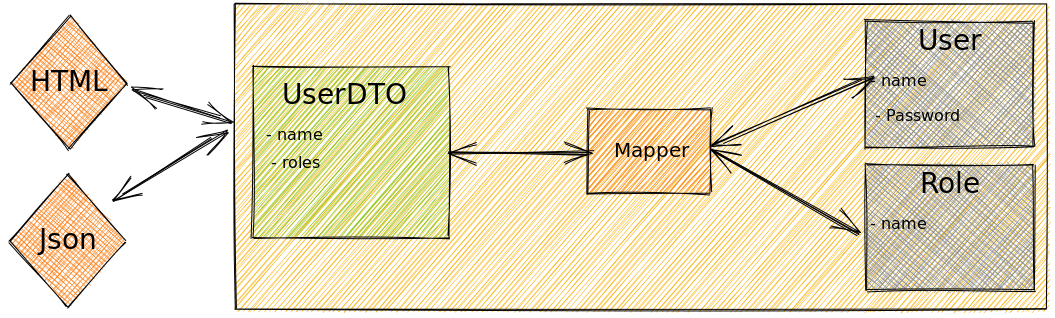
\includegraphics[width=0.7\textwidth]{dto.png}
    \caption{Esempio di utilizzo del \textit{design pattern} DTO}
    \small Fonte: \href{https://www.baeldung.com/java-dto-pattern} {www.baeldung.com}
    \label{fig:dto}
\end{figure}
\noindent
Un altro \textit{desig pattern} che ho utilizzato è il \textit{Mapper pattern}, che è strettamente collegato al \gls{dtog} \textit{pattern}.  Come mostro nell'immagine \ref{fig:dto}, il \textit{mapper} consiste in uno o più metodi per facilitare la trasformazione dei \gls{dtog} in oggetti utilizzati dalla logica di \textit{business}, mappando i diversi campi da un tipo all’altro. All'interno del sistema Jira, il \textit{mapper} è stato utilizzato per trasformare i dati ricevuti dalle \gls{apig} di Jira in oggetti \textit{ticket} che vengono utilizzati dalle funzioni \textit{lambda} per eseguire le operazioni di salvataggio e di richiesta di proposta di risoluzione.
Questo \textit{design pattern} contribuisce a mantere il codice organizzato, garantendo che i dati siano nel formato corretto. Ho adottato il \textit{Factory Method pattern} per la creazione delle interfacce di connessione con i vari modelli offerti da \gls{aws} Bedrock. Questo \textit{design pattern} permette di astrarre la logica di creazione degli oggetti, permettendo l'aggiunta di nuovi modelli senza la necessità di modificare il codice esistente. La flessibilità e la scalabilità
offerta da questo \textit{design pattern} sono state fondamentali per garantire che il sistema possa evolvere nel tempo, permettendo l'integrazione di nuovi modelli che verranno resi disponibili in futuro. 
\begin{figure}[H]
    \centering
    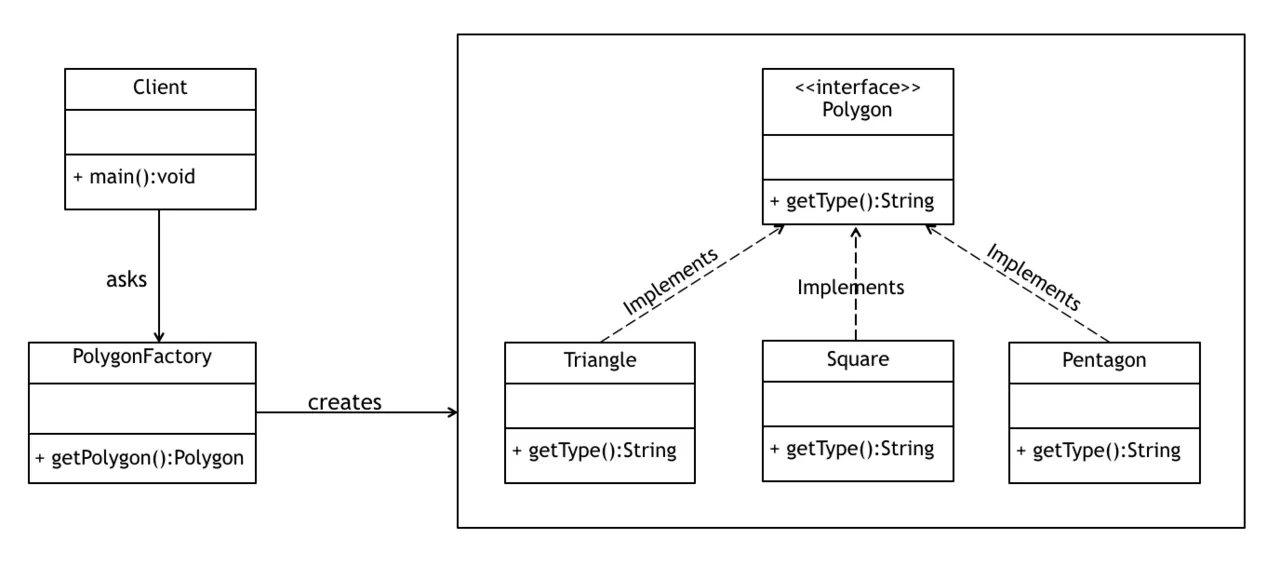
\includegraphics[width=0.7\textwidth]{factoryPattern.png}
    \caption{Illustrazione del \textit{design pattern} Factory Method}
    \small Fonte: \href{https://medium.com/@contactkumaramit9139/factory-design-pattern-in-java-baee365fc1ce} {www.medium.com}
    \label{fig:factory}
\end{figure}
\noindent
Infine, ho adottato il \textit{design pattern Strategy} per la creazione delle strategie di generazione del \textit{prompt} e di risposta dei vari \gls{llm} offerti da \gls{aws} Bedrock. Definisco una strategia di generazione \textit{prompt} ad ogni modello in quanto ognuno di essi possiede delle \textit{keywords} e una formattazione del testo specifico. Il \textit{prompt} mostrato nella sezione \ref{sec:rag} è la base per ognuno dei modelli. 

\begin{figure}[H]
    \centering
    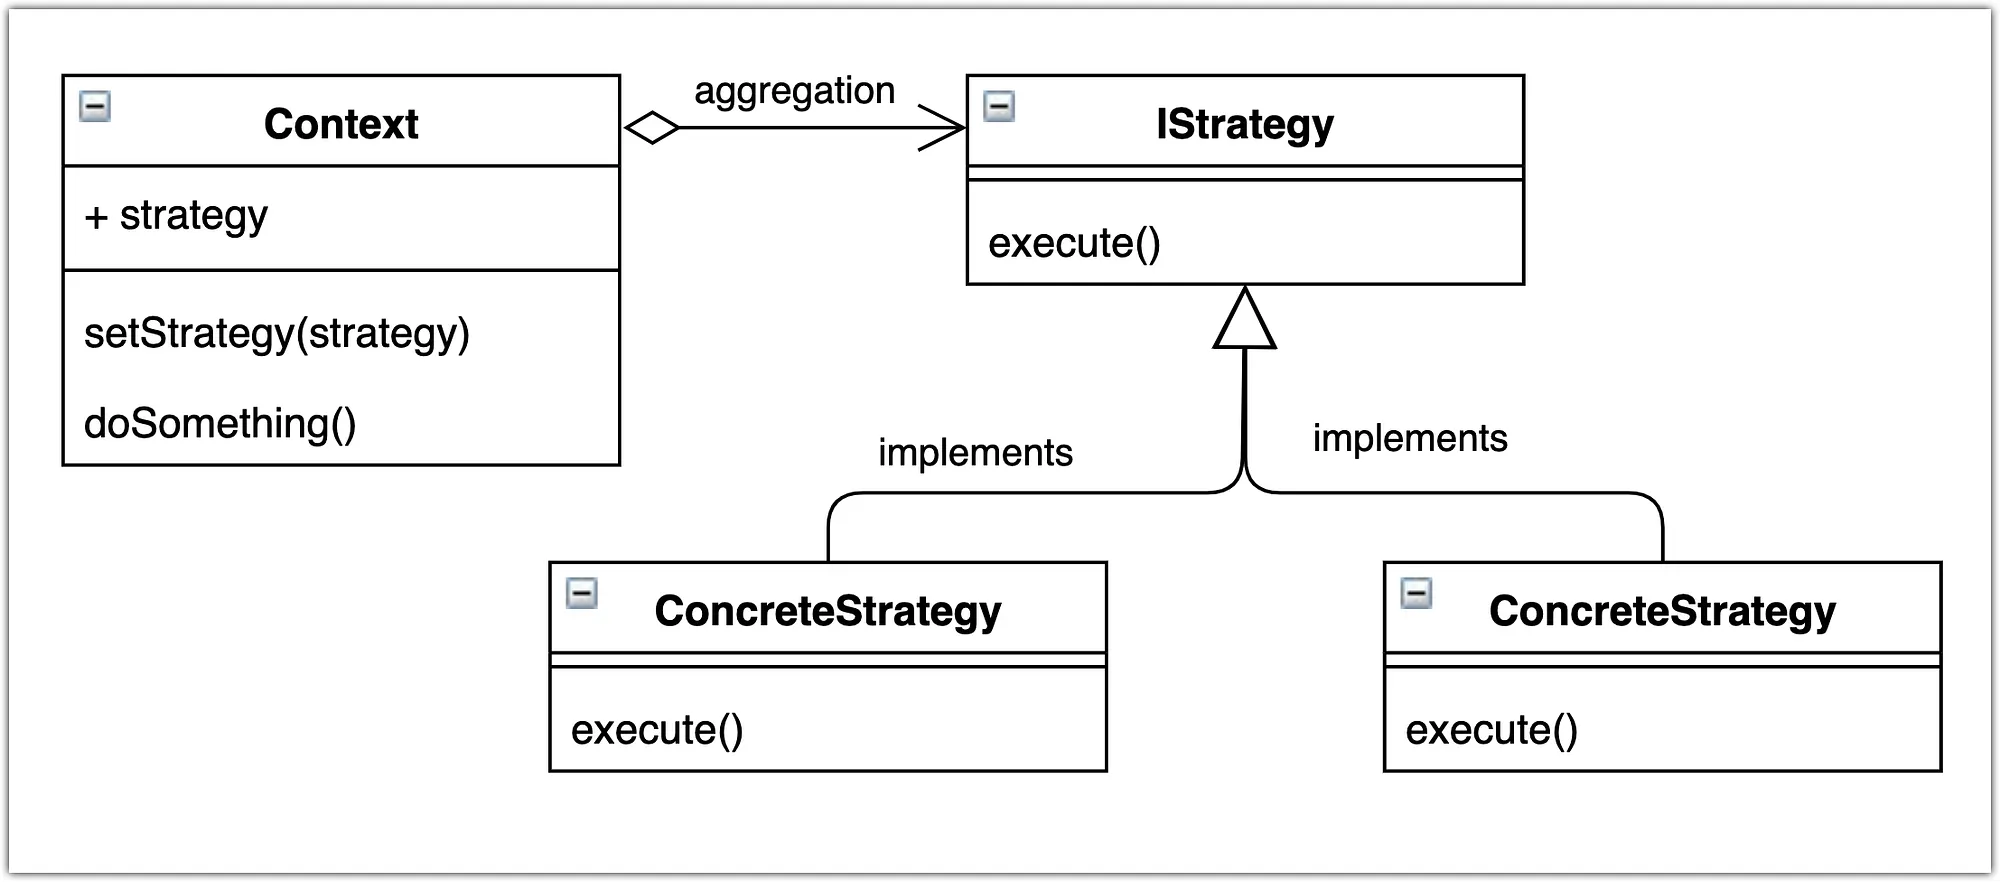
\includegraphics[width=0.7\textwidth]{strategy.png}
    \caption{Illustrazione del \textit{design pattern} Strategy}
    \small Fonte: \href{https://medium.com/litslink/design-patterns-strategy-in-examples-eae7bf10a817} {www.medium.com}
    \label{fig:strategy}
\end{figure}

\noindent
In figura \ref{fig:architetturaJira} mostro lo schema dell'architettura del sistema Jira:
\begin{figure}[H]
    \centering
    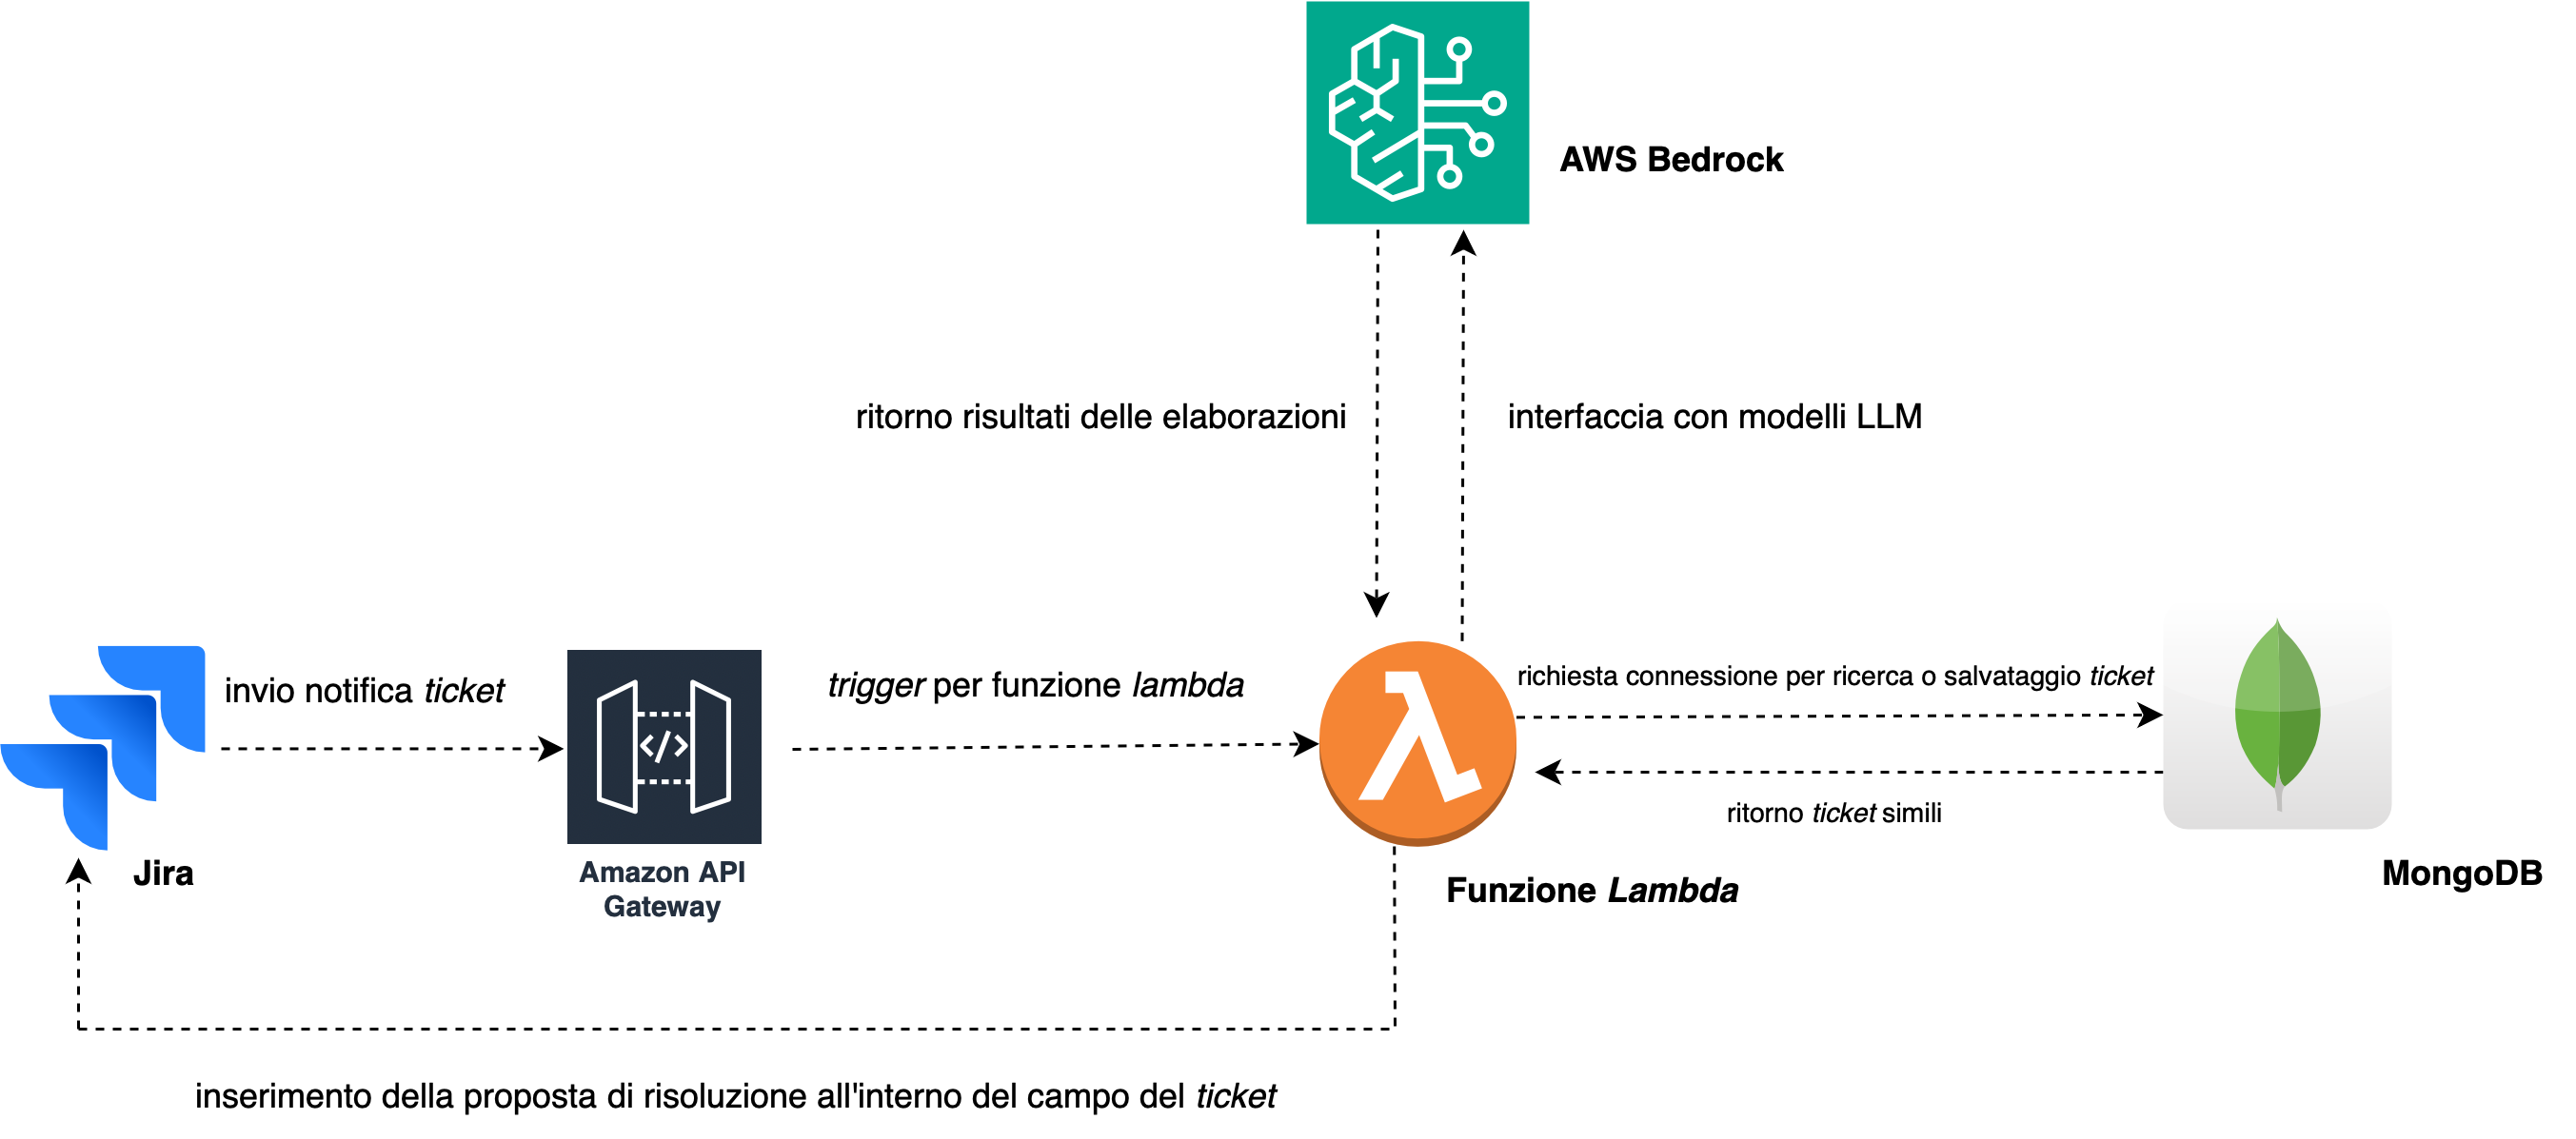
\includegraphics[width=0.95\textwidth]{architettura.png}
    \caption{Schema dell'architettura del sistema Jira}
    \label{fig:architetturaJira}
\end{figure}

\subsection{Architettura del \textit{Chatbot}}
La progettazione del \textit{chatbot} si è basata sull'architettura \textit{client-server} del \textit{framework} Streamlit. Il \textit{client} viene rappresentato dal \textit{browser} che l'utente utilizza per interagire con il \textit{chatbot}, mentre il \textit{server} è rappresentato dall'esecuzione del codice Python che in risposta alle azioni dell'utente, invia i risultati al \textit{client} sotto forma di \gls{htmlg}/\gls{cssg}/JavaScript che vengono visualizzati nel \textit{browser}.
\subsubsection{\textit{Back-end}}
Essendo l'architettura del \textit{chatbot} basata sul \textit{framework} Streamlit, il \textit{back-end} è rappresentato dal codice Python che viene eseguito in risposta alle azioni dell'utente.
Una componente chiave del \textit{back-end} è l'utilizzo del \textit{framework} Langchain. Esso viene impiegato in diverse parti cruciali del \textit{back-end}, ovvero:
\begin{itemize}
    \item \textbf{Integrazione con il \textit{database} vettoriale}: con l'utilizzo di Langchain, è possibile stabilire una connessione con il \textit{database} vettoriale MongoDB per effettuare la ricerca vettoriale dei \textit{ticket} completati più simili al testo inserito dall'utente;
    \item \textbf{Gestione degli \gls{embedding-g}}: tramite LangChain viene facilitato l'uso di diversi modelli di \gls{embedding-g} messi a disposizione da \gls{aws}. 
    \item \textbf{Orchestrazione dei modelli}: come da requisito da soddisfare presentato nella tabella \ref{tab:tracciamentoRequisiti}, il \textit{chatbot} deve poter dare la possibilità all'utente di selezionare l' \gls{llm} con cui interrogare il \textit{chatbot}. LangChain permette di integrare ed orchestrare i diversi modelli consentendo una flessibilità nella scelta e nell'utilizzo dei modelli scelti dall'utente.
\end{itemize} 
\noindent
Anche in questo caso ho adotatto il \textit{Factory Method pattern} per la creazione delle interfacce di connessione con i vari modelli offerti da \gls{aws} Bedrock e il \textit{design pattern Strategy} per la creazione delle strategie di generazione del \textit{prompt}.
\subsubsection{\textit{Front-end}}
Allo stesso modo, il \textit{front-end} del \textit{chatbot} è anch'esso rappresentato da codice Python. Tramite la libreria Streamlit, è possibile creare un'interfaccia grafica interattive per l'utente. Possiede una serie di componenti per la creazione di \textit{widget}. Grazie all' utilizzo \textit{framework}, l'interfaccia viene aggiornata automaticamente in risposta alle azioni dell'utente. \\ \\
\noindent
In figura \ref{fig:architetturaChatbot} mostro lo schema dell'architettura del \textit{chatbot}:
\begin{figure}[H]
    \centering
    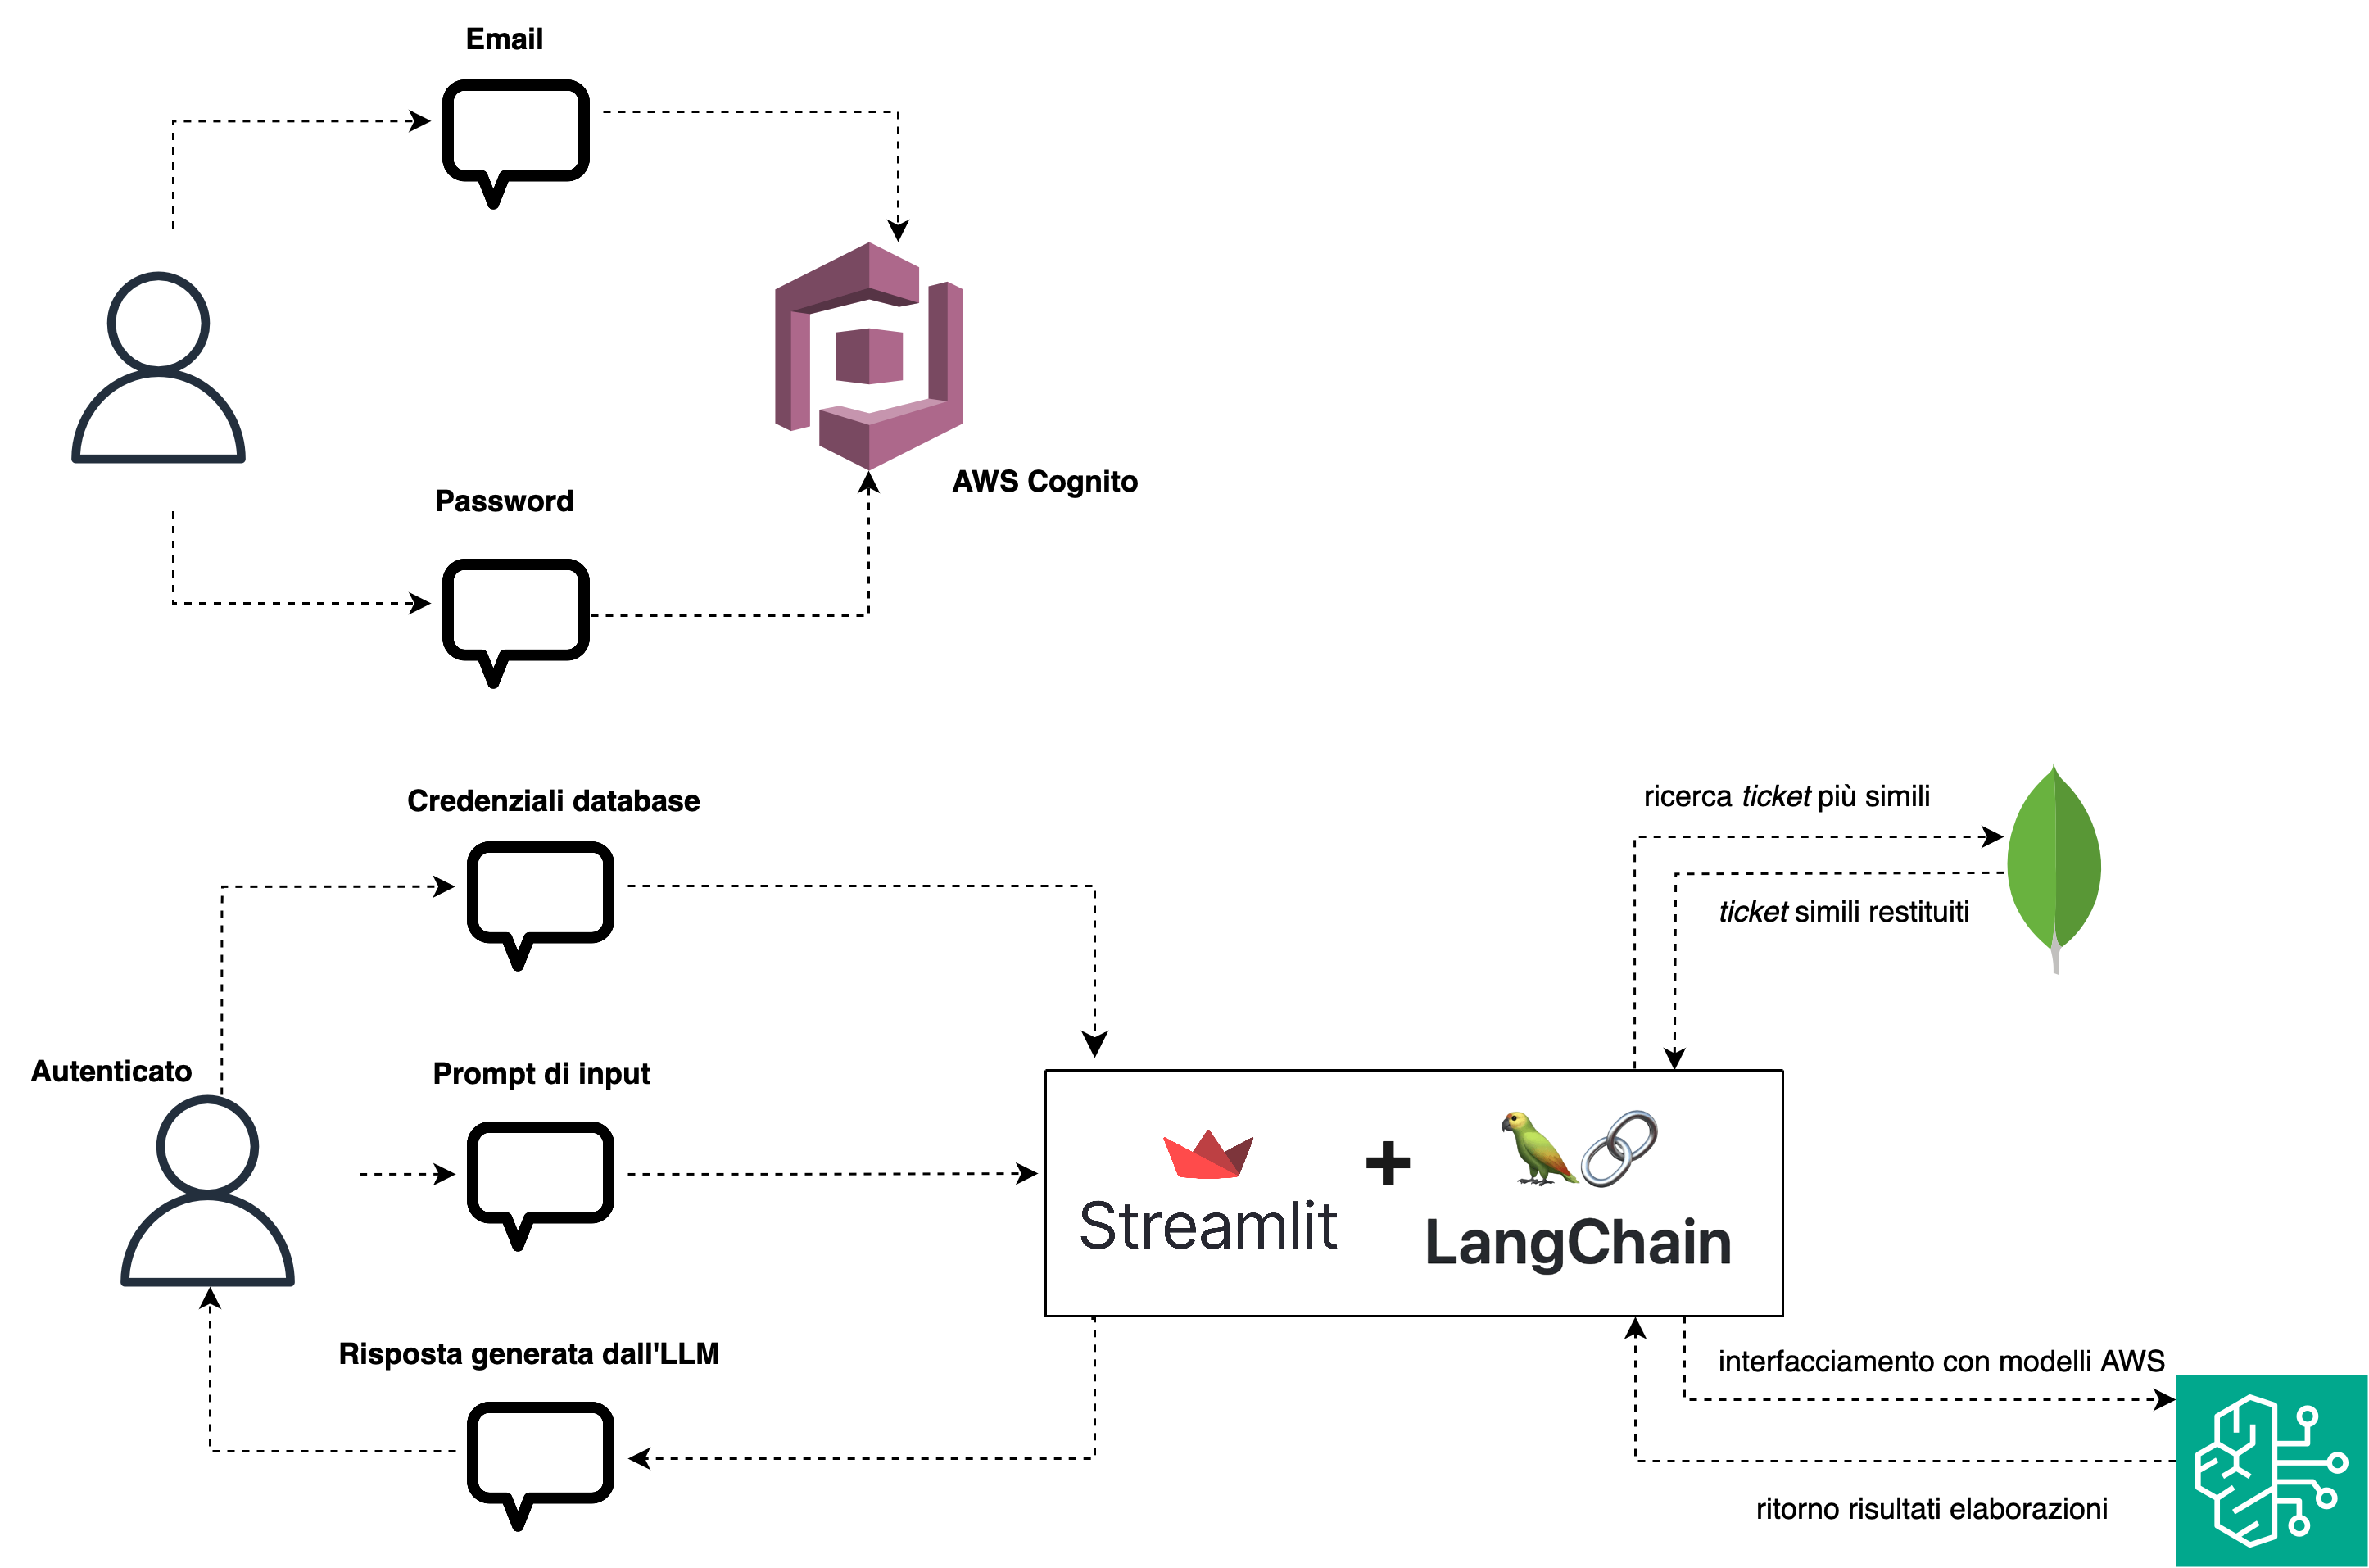
\includegraphics[width=0.95\textwidth]{chatbot_architettura.png}
    \caption{Schema dell'architettura del \textit{chatbot}}
    \label{fig:architetturaChatbot}
\end{figure}

\section{Codifica}
\subsection{Sistema Jira}

Al fine di sviluppare un sistema con le funzionalità definite durante il processo di progettazione, ho sviluppato due \textit{handlers} (ovvero due funzioni \textit{lambda}), che descrivo qui di seguito:

\begin{itemize}
    \item \textbf{\textit{suggest}}: funzione \textit{lambda} che viene eseguita quando un evento \gls{httpg} viene scatenato da \gls{aws} API Gateway. Questo evento si verifica quando un \textit{ticket} viene creato, attraverso i \textit{webhook} di Jira. La funzione \textit{suggest} si occupa di interrogare il \textit{database} vettoriale per la ricerca dei \textit{ticket} più simili al \textit{ticket} appena creato e di generare una proposta di risoluzione utilizzando l'\gls{llm} impostato. La proposta di risoluzione viene poi inserita all'interno di un campo personalizzato dedicato al \textit{ticket} creato in Jira.
    All'interno della funzione \textit{suggest}, ho sviluppato delle funzioni \textit{services} che si occupano di effettuare la ricerca vettoriale, di interrogare l'\gls{llm} e di generare la proposta di risoluzione. Questo approccio permette di mantenere il codice pulito e organizzato, garantendo che ogni funzione abbia un compito specifico e ben definito.
    \begin{minted}[fontsize=\small,breaklines, linenos, numbersep=5pt, frame=lines, framesep=2mm]{typescript}
async function handler(event: Event<TicketDataEventDto>): Promise<undefined> {
    if (!isDefined(event.body)) {
        throw new HTTP400Error('Il body e\' undefined');
    }
    const body: TicketDataEventDto = event.body;
    const ticket: Ticket = await createTicket(body);

    if (isDefined(ticket) && ticket.status === 'Open') {
        const embeddingService: EmbeddingModel = createEmbeddingModels('AmazonTitanV2');
        await suggestSolution(ticket, ticket.key, embeddingService);
    } else {
        throw new Error('Errore nella pipeline di elaborazione del ticket');
    }
}

export const main: HandlerResponse = baseHandler<TicketDataEventDto, undefined>(handler, 200);
    \end{minted}
    \captionof{figure}{Funzione \textit{lambda suggest}}

    \item \textbf{\textit{save}}: funzione \textit{lambda} che viene eseguita quando un evento \gls{httpg} viene scatenato da \gls{aws} API Gateway. Questo evento si verifica quando un \textit{ticket} viene chiuso, sempre con l'ausilio dei \textit{webhook} di Jira. La funzione \textit{save} si occupa di salvare il \textit{ticket} chiuso e il suo relativo \gls{embedding-g} all'interno del \textit{database}. Questo permette di poter ricercare in futuro i \textit{ticket} completati più simili ai \textit{ticket} creati, arricchendo così la conoscenza del \textit{database}.
    Anche in questo caso, ho sviluppato delle funzioni \textit{services} che si occupano di inserire il \textit{ticket} chiuso e di calcolare il relativo \gls{embedding-g} all'interno del \textit{database}.
    \begin{minted}[fontsize=\small,breaklines, linenos, numbersep=5pt, frame=lines, framesep=2mm]{typescript}
async function handler(event: Event<TicketDataEventDto>): Promise<undefined> {
    if (!isDefined(event.body)) {
        throw new HTTP400Error('Il body e\' undefined');
    }
    const body: TicketDataEventDto = event.body;
    const ticket: Ticket = await createTicket(body);
    
    const embeddingService: EmbeddingModel = createEmbeddingModels('AmazonTitanV2');
    
    if (isDefined(ticket) && ticket.status === 'Done') {
        await processEmbedding(ticket, embeddingService, false);
        await saveTicket(ticket);
    } else {
        throw new Error('Errore nella pipeline di elaborazione del ticket');
    }
}

export const main: HandlerResponse = baseHandler<TicketDataEventDto, undefined>(handler, 200);
    \end{minted}
    \captionof{figure}{Funzione \textit{lambda save}}
\end{itemize}


\subsection{\textit{Chatbot}}
Per lo sviluppo del \textit{chabot} come ho descritto precedentemente ho utilizzato il \textit{framework} Streamlit. Questo \textit{framework} mi ha permesso di sviluppare il \textit{back-end} e il \textit{front-end} del \textit{chatbot} in semplici \textit{file} Python.
Qui di seguito descrivo la suddivisione dei \textit{file} Python che compongono il \textit{chatbot}:
\begin{itemize}
    \item \textbf{\textit{Back-end}}: per quanto riguarda il \textit{back-end} del \textit{chatbot}, ho creato diversi \textit{file} Python che si occupano di gestire l'\textit{input} dell'utente, di interrogare il \textit{database} vettoriale per la ricerca dei \textit{ticket} più simili e l'interfacciamento con i vari modelli \gls{llm} offerti da \gls{aws} Bedrock. Ho gestito queste diverse operazioni con l'ausilio del \textit{framework} LangChain. Qui di seguito mostro un esempio di uno dei \textit{file} Python che compongono il \textit{back-end} del \textit{chatbot}.
    \begin{minted}[fontsize=\small,breaklines, linenos, numbersep=5pt, frame=lines, framesep=2mm]{python}

from langchain_community.vectorstores import MongoDBAtlasVectorSearch

def cloudVectorSearch(database_url, database_name, collection_name, query_embedding):
    namespace = f"{database_name}.{collection_name}"

    vector_search = MongoDBAtlasVectorSearch.from_connection_string(
        database_url,
        namespace,
        embeddings,
        embedding_key="embedding",
        index_name="vector_index",
        text_key="raw"
    )
    search_result = vector_search.similarity_search_with_relevance_scores(
        query_embedding,
        k=3,
    )

    desired_fields = ['key','summary', 'description', 'resolution_description', 'components']
    filtered_result = filter_fields(search_result, desired_fields)

    return filtered_result
    \end{minted}
    \captionof{figure}{Funzione di ricerca vettoriale utilizzata nel \textit{chatbot}}
    \label{lst:cloudVectorSearch}


    Nel frammento di codice \ref{lst:cloudVectorSearch} mostro la funzione di ricerca vettoriale utilizzata nel \textit{chatbot}. Questa funzione si occupa di interrogare il \textit{database} vettoriale MongoDB fornendogli il nome dell'indice, il nome del campo contenente l'\gls{embedding-g} e l'\gls{embedding-g} del testo della \textit{query} dell'utente. La funzione restituisce i tre \textit{ticket} più simili alla \textit{query} dell'utente filtrandoli per i campi desiderati.
    \item \textbf{\textit{Front-end}}: per lo sviluppo del \textit{front-end} del \textit{chatbot} ho creato un unico \textit{file} Python che si occupa di creare l'interfaccia grafica interattiva utilizzando le componenti offerte dal \textit{framework} Streamlit. Questo \textit{file} Python si occupa di gestire l'interfaccia grafica, di inviare le richieste al \textit{back-end} e di visualizzare i risultati all'utente.
    \begin{minted}[fontsize=\small,breaklines, linenos, numbersep=5pt, frame=lines, framesep=2mm]{python}
input_text = st.chat_input()

if input_text:
    with st.chat_message("user"):
        st.write(input_text)

    st.session_state.chat_history.append(HumanMessage(input_text))

        search_result = cloudVectorSearch(st.session_state['database_url'], st.session_state['database_name'], st.session_state['collection_name'], input_text)
    else:
    st.session_state.search_results.append(search_result)

    with st.chat_message("assistant"):
        chat_response= st.write_stream(conversation(input_text, st.session_state.chat_history,
        st.session_state.search_results, model_choice))
    st.session_state.chat_history.append(AIMessage(chat_response))
    \end{minted}
    \captionof{figure}{Frammento del codice Python relativo al \textit{front-end}}
    \label{lst:chatbotFrontend} 

    Nel frammento di codice \ref{lst:chatbotFrontend} mostro un esempio di come viene gestita la richiesta dell'utente e come vengono visualizzati i relativi risultati. Viene effettuata una ricerca vettoriale che restituisce i \textit{ticket} più simili alla \textit{query} dell'utente. 
    Successivamanete inserisco i risultati all'interno della \textit{st.session\_state} che rappresenta la sessione dell'utente. Infine viene generata la proposta di risoluzione con l'ausilio del \gls{llm} scelto dall'utente con i risultati della ricerca vettoriale e visualizzata all'utente.
\end{itemize}

\subsection{\textit{Best practice}}
Durante il mio periodo di \textit{stage} ho fatto uso di diversi strumenti utilizzati in ambito aziendali e ho potuto apprendere alcune \textit{best practice} che ho applicato durante l'attività di codifica per lavorare allo stato dell'arte. Di seguito elenco alcune delle \textit{best practice} che ho applicato:
\begin{itemize}
    \item \textbf{\textit{Editor} di codice}: all'inzio dell'attività di codifica mi è stato richiesto di utilizzare la configurazione aziendale del \textit{plugin} ESLint. Come ho descritto in \ref{sec:tecnologie}, ESLint è uno strumento di analisi statica del codice che permette di identificare e segnalare gli errori di sintassi e di stile presenti nel codice.  Questo strumento mi ha permesso di scrivere codice uniforme e pulito, seguendo lo \textit{standard} aziendale. Inoltre, ha permesso di ridurre il numero di errori di sintassi e di stile presenti nel codice, velocizzando le \textit{code review} necessarie per l'avanzamento del progetto.
    \item \textbf{\textit{Code reviews}}: l'intera attività di codifica è stata sottoposta a \textit{code reviews} da parte del mio \textit{tutor} aziendale e da un altro membro dell'azienda. Anche in questo caso mi sono attenuto al processo già ben consolidato in azienda. Per ogni funzionalità sviluppata, ho creato una \textit{feature \gls{branch-g}} all'interno di un \textit{repository} Git dedicato. Il \textit{feature \gls{branch-g}} veniva denominato con la seguente notazione:
    \begin{center}
        \textbf{\emph{feature/nome\_funzionalità}}
    \end{center}
    in modo da rendere chiaro il contenuto del \textit{\gls{branch-g}}. Una volta che completavo lo sviluppo della funzionalità, aprivo una \textit{\gls{pull-request-g}} per la \textit{code review}. Questo processo mi ha permesso di ricevere \textit{feedback} costante sul codice che stavo sviluppando, permettondomi di correggere eventuali errori e di migliorare la qualità del codice. Infine, mi ha permesso di approfondire in modo più dettagliato l'utilizzo di Github come strumento di versionamento del codice e di osservare come si sviluppa codice seguendo dei processi consolidati e ben definiti.
    \item \textbf{\textit{Interfaces}}: Typescrit richiede la dichiarazione esplicita dei tipi delle variabili e degli oggetti utilizzati all'interno del codice. Per questo motivo, ho definito delle \textit{interfaces} per definire i tipi di tutti gli oggetti utilizzati a cui non potevano essere assegnati i tipi primitivi. A differenza delle classi, le \textit{interfaces} non vengono instanziate, ma presentano solo i tipi degli attributi e la firma dei metodi che un oggetto avrà una volta implementato. Questo mi ha permesso di definire in modo chiaro e preciso i tipi degli oggetti utilizzati all'interno del codice, in modo da non incorrere in errori di tipo durante l'esecuzione del codice.
    \item \textbf{Documentazione}: durante tutta l'attività di codifica ho documentato il codice sviluppato attraverso l'utilizzo di commenti. Durante l'ultima settimana di \textit{stage} ho redatto una documentazione tecnica dettagliata contenente le scelte progettuali fatte per entrambi i progetti, con le funzionalità implementate, e un manuale utente per il corretto utilizzo del sistema Jira e del \textit{chatbot}. 
\end{itemize}

\section{Verifica e validazione}
\subsection{Sistema Jira}
\subsubsection{\textit{Test} tramite eventi}
Per verificare il corretto funzionamento delle due funzioni \textit{lambda} che ho sviluppato per il sistema Jira, ho utilizzato il servizio di \textit{testing} tramite eventi offerto da \gls{aws} Lambda. Tramite questo servizio ho potuto creare un evento di test che simulava l'evento scatenato da \gls{aws} API Gateway quando un \textit{ticket} viene creato o chiuso. Tramite questo approccio ho potuto verificare che le funzioni \textit{lambda} ricevessero correttamente il \textit{ticket} dall'evento. Le operazioni di proposta di risoluzione e di salvataggio del \textit{ticket} sono state testate a parte, in quanto richiedevano l'interrogazione del \textit{database} vettoriale e l'interfacciamento con i vari modelli \gls{llm} offerti da \gls{aws} Bedrock. 
\begin{figure}[H]
    \centering
    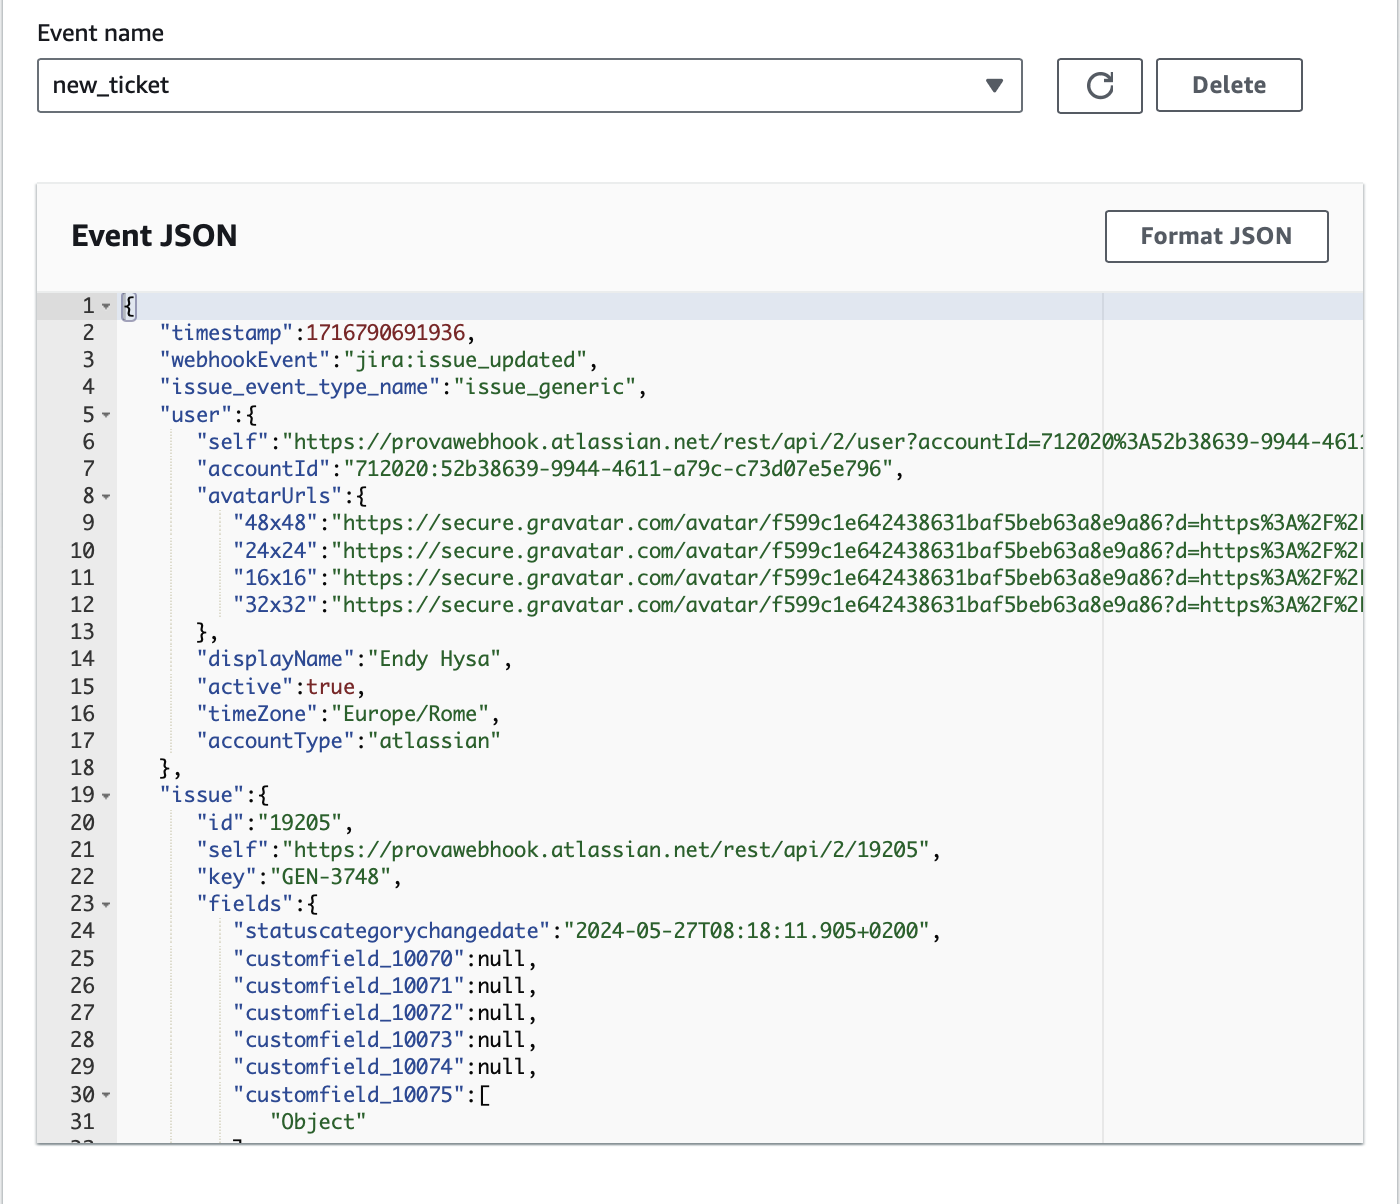
\includegraphics[width=0.65\textwidth]{eventTest.png}
    \caption{Esempio di evento di \textit{test}}
    \label{fig:testLambda}
\end{figure}
\noindent
Nell'immagine \ref{fig:testLambda} mostro un esempio di evento di test creato per verificare il corretto funzionamento della funzione \textit{lambda} \textit{suggest}. L'evento contiene i dati di un \textit{ticket} fittizio creato per il \textit{testing}. Tramite questo evento ho potuto verificare che il \textit{ticket} contenuto nell'evento venisse correttamente ricevuto dalla funzione \textit{lambda}.

\subsubsection{\textit{Test} di integrazione}
I \textit{test} di integrazione si occupano di verificare che le varie componenti del sistema funzionino correttamente, garantendo che le varie parti dell'applicativo interagiscano nel modo corretto. Durante il mio periodo di \textit{stage} ho potuto svolgere i \textit{test} di integrazione per verificare che le due funzioni \textit{lambda} sviluppate per il sistema Jira interagissero correttamente con il \textit{database} vettoriale e con l'\gls{llm} impostato per la generazione delle proposte di risoluzione. 
Questi \textit{test} li ho svolti manualmente. Il \textit{framework} Serverless offre la possibilità di esporre le funzioni \textit{lambda} in locale, chiamabili tramite \gls{api} con il comando \textit{serverless-offline}. Questo mi ha permesso di simulare l'interazione tra le varie componenti e servizi del sistema Jira, testati attraverso Postman. Come descritto nella sezione \ref{sec:tecnologie}, Postman è uno strumento di \textit{testing} delle \gls{api} che permette di effettuare richieste \gls{httpg} e di verificare le risposte ricevute.

\noindent
Con i \textit{test} di integrazione si conclude il processo di verifica e validazione del sistem Jira, che mi ha permesso di verificare il corretto funzionamento del prodotto sviluppato e che soddisfi le aspettative dell'azienda.

\subsection{\textit{Chatbot}}
Per quanto riguarda il \textit{chatbot}, ho svolto solamente i \textit{test} di integrazione. Questi \textit{test} li ho svolti manualmente per verificare che il \textit{chatbot} funzionasse correttamente e che le varie componenti interagissero nel modo corretto.
Essendo nata l'idea di sviluppare il \textit{chatbot} durante il mio periodo di \textit{stage}, non è stato possibile dedicare molto tempo alla creazione di \textit{test}, in quanto il suo scopo principale era quello di dimostrare la fattibilità e l'utilità di un \textit{chatbot} per l'interrogazione dei \textit{ticket} di Jira.
\section{Risultato finale}
\subsection{Il prodotto realizzato}
I prodotti che ho realizzato durante il mio periodo di \textit{stage} soddisfano quanto atteso dall'azienda, risultando funzionanti e rispettando i requisiti richiesti. 
\subsection*{Sistema Jira}
Quando l'utente si sarà autenticato nel \textit{workspace} Jira, potrà creare un \textit{ticket} e il sistema da me sviluppato si occuperà di generare una proposta di risoluzione per il \textit{ticket} creato
\begin{figure}[H]
    \centering
    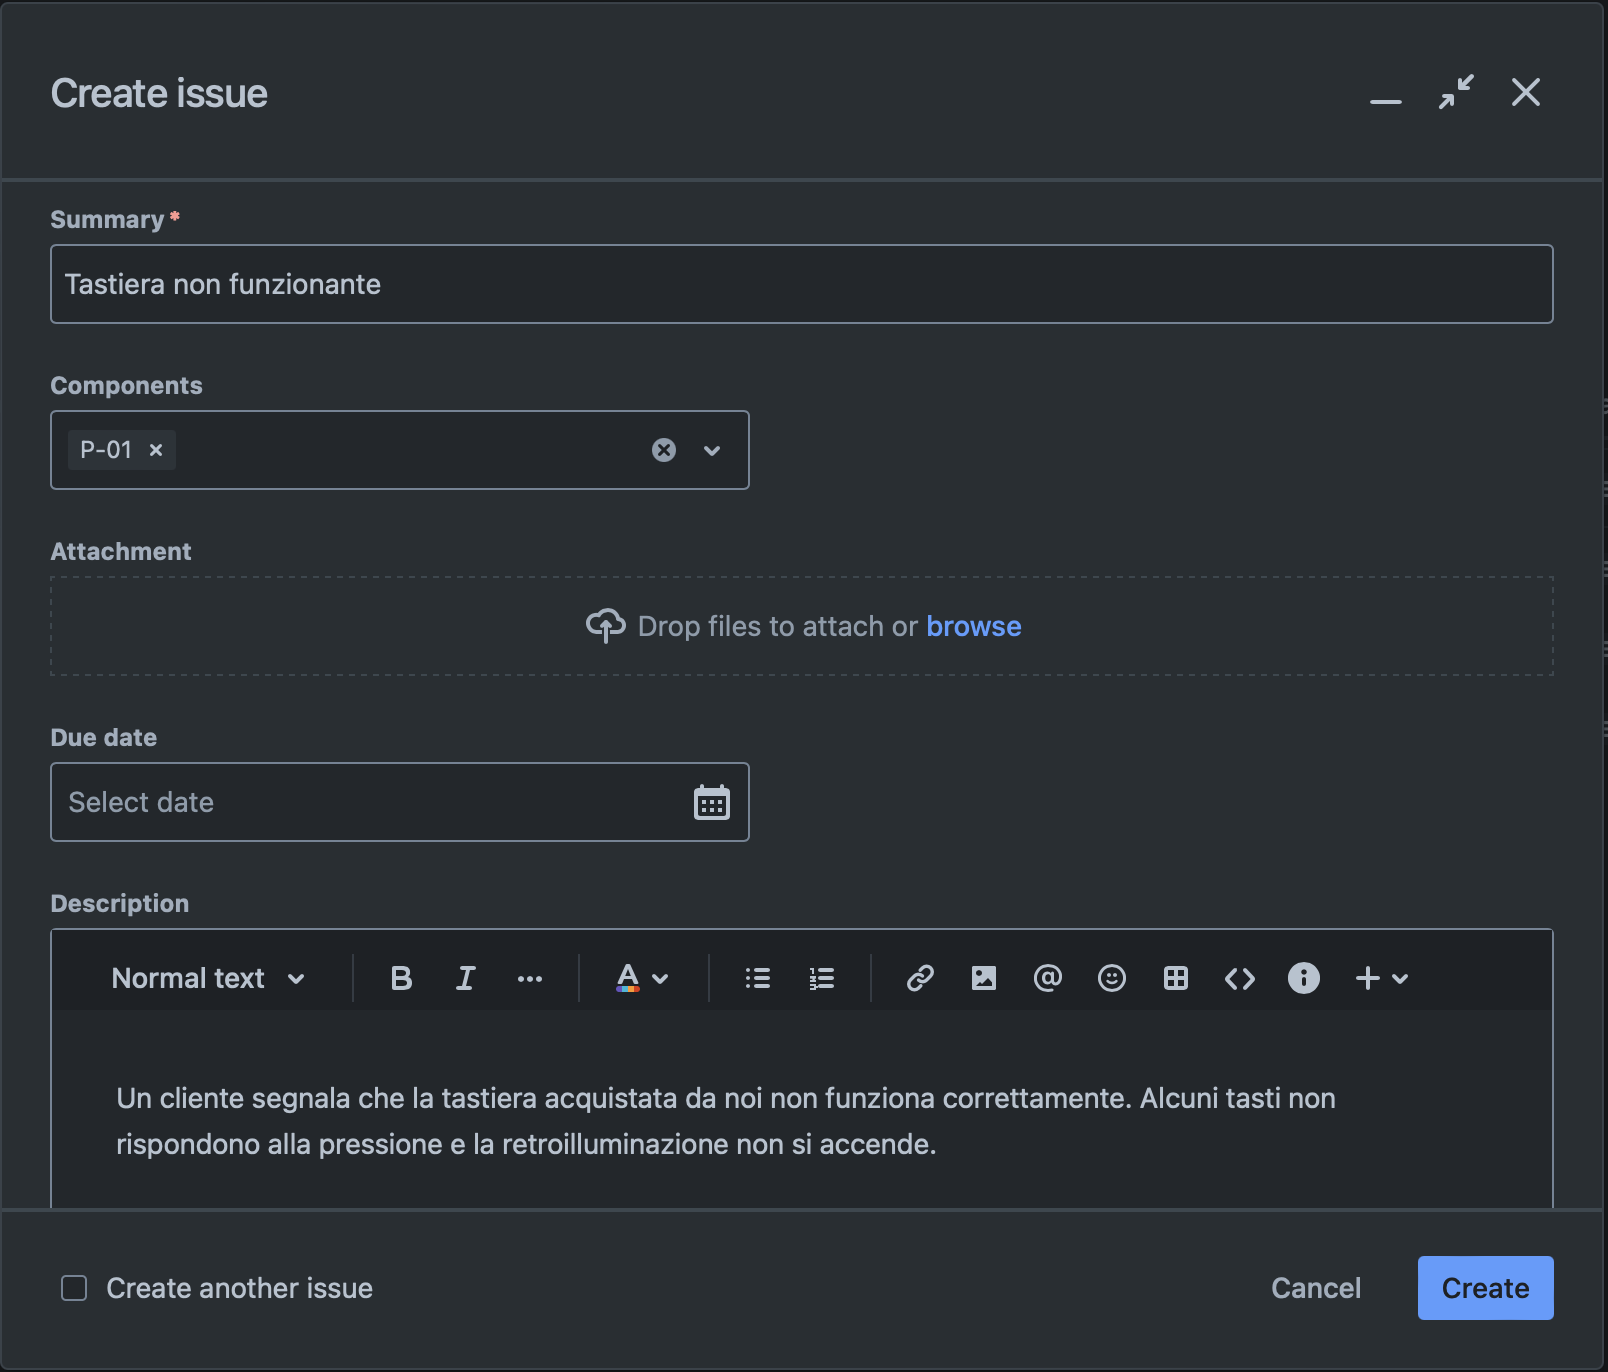
\includegraphics[width=0.78\textwidth]{create_Issue.png}
    \caption{Creazione di un nuovo \textit{ticket} su Jira} 
    \label{fig:creazioneTicket}
\end{figure}
\noindent
Come mostro nell'immagine \ref{fig:creazioneTicket}, l'utente premendo il pulsante \textit{Create}, creerà un nuovo \textit{ticket} su Jira con i relativi campi compilati. Una volta creato il \textit{ticket}, il sistema Jira comincerà a generare una proposta di risoluzione per il \textit{ticket} creato.
\begin{figure}[H]
    \centering
    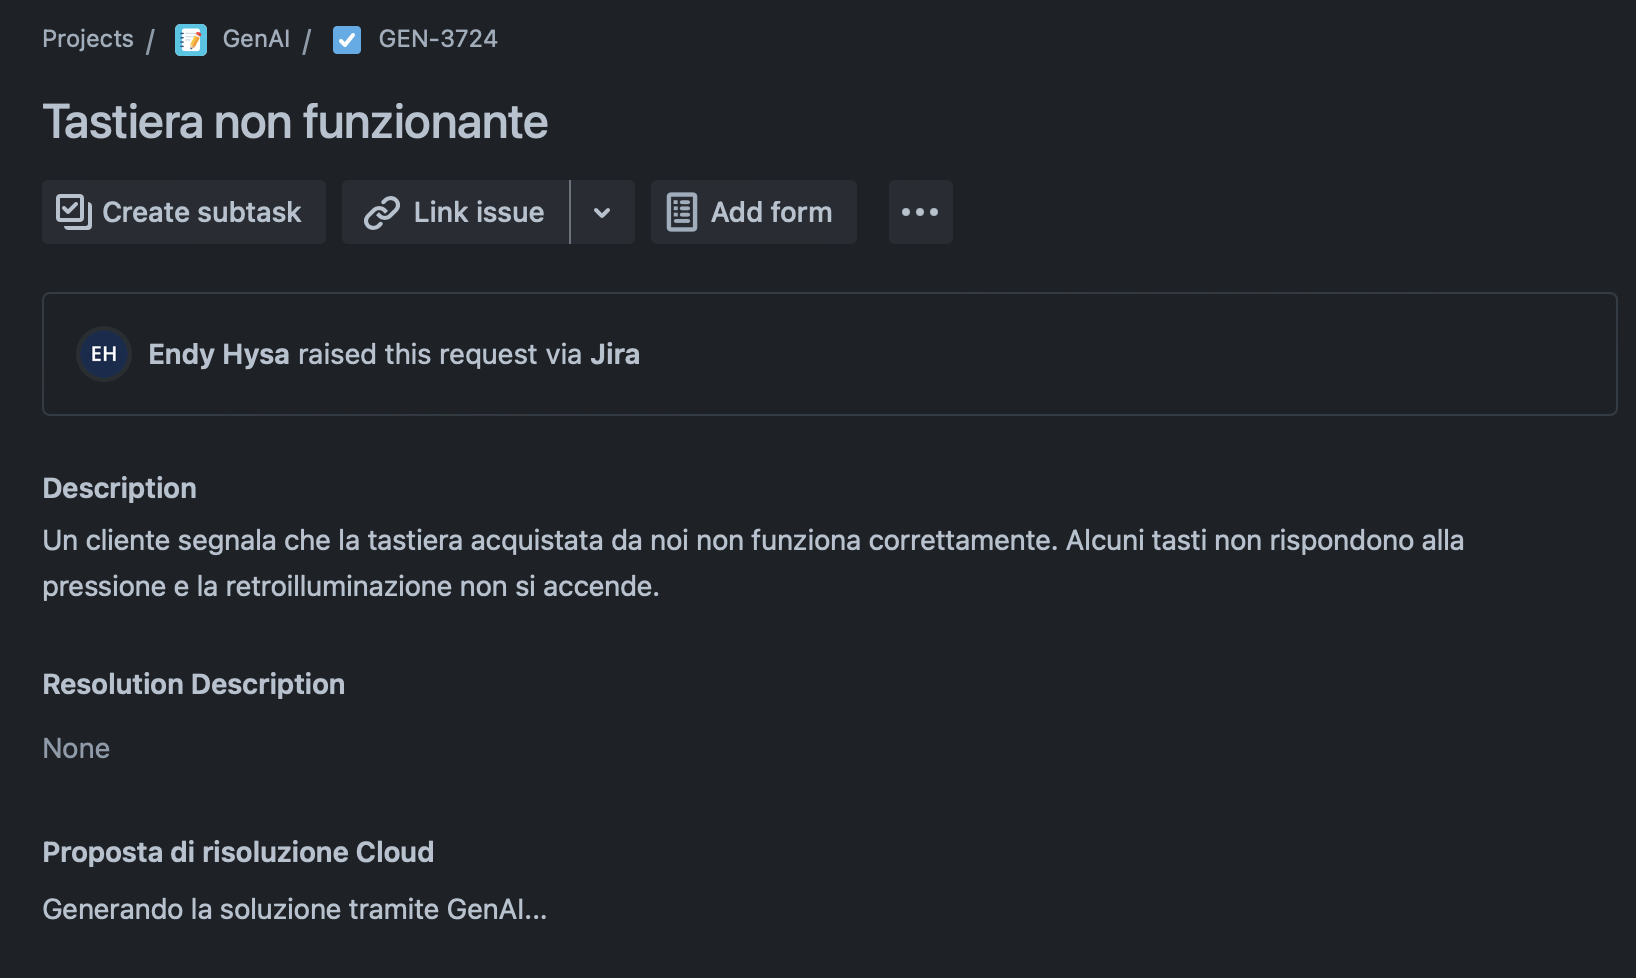
\includegraphics[width=0.85\textwidth]{generatingResponse.png}
    \caption{Messaggio che indica che il sistma sta generando la proposta di risoluzione} 
    \label{fig:generatingResponse}
\end{figure}
\noindent
Nell'immagine \ref{fig:generatingResponse} mostro il messaggio che indica che il sistema sta generando la proposta di risoluzione per il \textit{ticket} creato. Una volta che la proposta di risoluzione è stata generata, sovrascriverà il messaggio di generazione.
\begin{figure}[H]
    \centering
    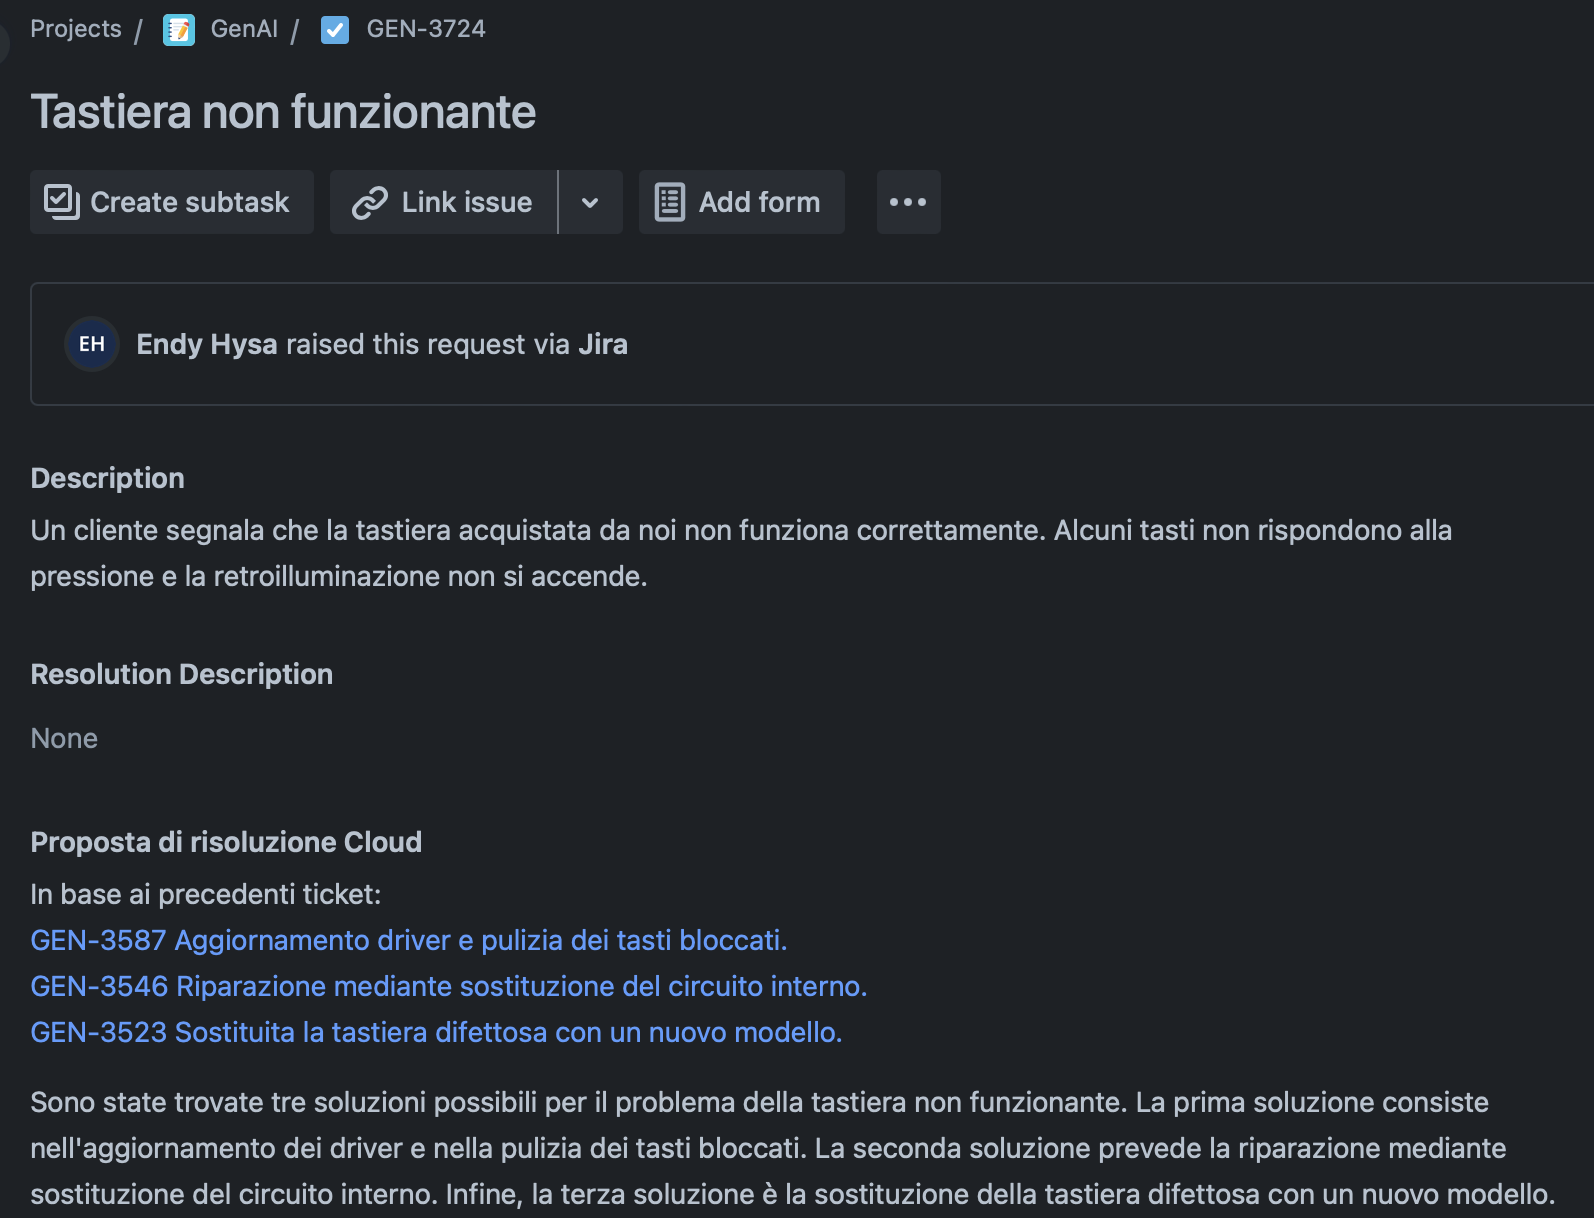
\includegraphics[width=0.85\textwidth]{responseGenerated.png}
    \caption{Proposta di risoluzione generata dal sistema ed inserita nel \textit{ticket} Jira}
    \label{fig:responseGenerated}
\end{figure}
\noindent
La proposta di risoluzione che mostro nell'immagine \ref{fig:responseGenerated}, che viene generata è inerente al \textit{ticket} creato e ai \textit{ticket} completati più simili. Nella proposta di risoluzione vengono inseriti anche i \textit{link} ai \textit{ticket} completati più simili, in modo da poterli consultare per avere ulteriori informazioni sulla risoluzione del problema.
Nel caso in cui l'utente crei un \textit{ticket} e le informazioni contenute non siano inerenti al problema, la proposta di risoluzione generata dal sistema Jira dichiarerà che non è possibile generare una proposta di risoluzione in quanto non sono presenti informazioni sufficienti.
\begin{figure}[H]
    \centering
    
\includegraphics[width=0.9\textwidth]{noResponse.png}
    \caption{Messaggio che indica che non è possibile generare una proposta di risoluzione}
    \label{fig:noResponse}
\end{figure}
\noindent
Nell'immagine \ref{fig:noResponse} mostro il messaggio che indica che non è possibile generare una proposta di risoluzione per il \textit{ticket} aperto. Questo viene mostrato in quanto il \textit{database} non contiene \textit{ticket} completati simili a quello aperto e pertanto non è possibile generare una proposta di risoluzione.\\
Mettendo il \textit{ticket} in stato \textit{Done}, il sistema Jira chiederà di inserire una risoluzione per il \textit{ticket} chiuso. Una volta inserita la risoluzione, il sistema Jira si occuperà di salvare il \textit{ticket} chiuso e il suo relativo \gls{embedding-g} all'interno del \textit{database} vettoriale. Questo viene fatto per arricchire la conoscenza del \textit{database} e permettere di poter ricercare i \textit{ticket} completati più simili ai \textit{ticket} creati in futuro.
\begin{figure}[H]
    \centering
    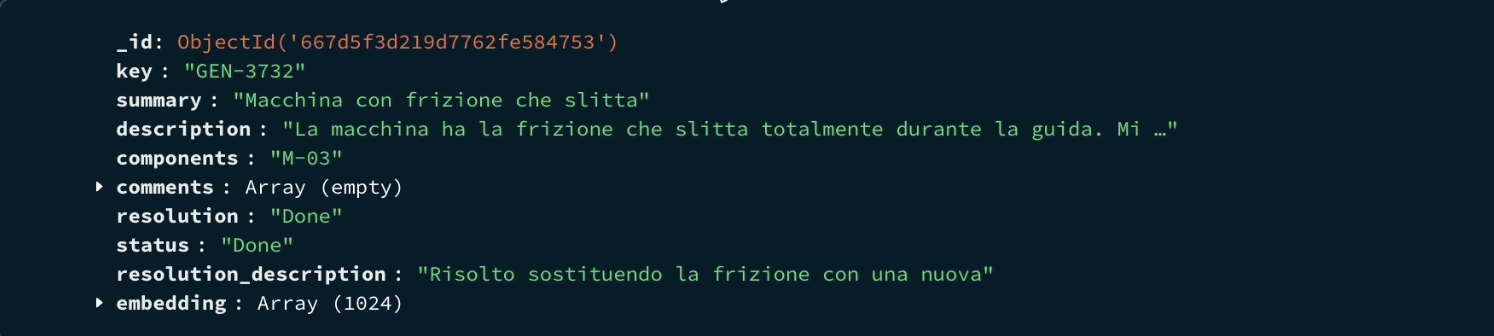
\includegraphics[width=0.9\textwidth]{closed.png}
    \caption{Schermata raffigurante il \textit{ticket} chiuso in MongoDB}
    \label{fig:closeIssue}
\end{figure}



\subsection*{\textit{Chatbot}}
Per poter interagire con il \textit{chatbot} che ho sviluppato durante il mio periodo di \textit{stage}, l'utente dovrà accedere tramite credenziali al \textit{chatbot} stesso. 
Come descritto nei requisiti di vincolo descritti nella tabella \ref{tab:tracciamentoRequisiti}, l'autenticazione avviene tramite \gls{aws} Cognito. 
\begin{figure}[H]
    \centering
    \includegraphics[width=0.7\textwidth]{beforeSignIn.png}
    \caption{Schermata di login del \textit{chatbot}}
    \label{fig:loginChatbot}
\end{figure}
\noindent
Una volta che l'utente si sarà autenticato, dovrà inserire le credenziali di accesso al \textit{database} vettoriale MongoDB. Questo passaggio è necessario per poter effettuare la ricerca vettoriale dei \textit{ticket} completati più simili a quello inserito dall'utente.
\begin{figure}[H]
    \centering
    \includegraphics[width=0.85\textwidth]{afterSignIn.png}
    \caption{Schermata di \textit{login} del \textit{chatbot}}
    \label{fig:afterSignIn}
\end{figure}
\noindent
Inserite dall'utente le credenziali necessarie, il \textit{chatbot} è pronto per essere utilizzato. L'utente potrà inserire il testo del \textit{ticket} di cui vuole avere una proposta di risoluzione e selezionare l'\gls{llm} con cui interrogare il \textit{chatbot}. L'utente dovrà inserire oltre alla problematica del \textit{ticket}, anche la sua relativa componente. Questo è necessario per poter effettuare una ricerca vettoriale più precisa e ottenere una proposta di risoluzione di qualità.
\begin{figure}[H]
    \centering
    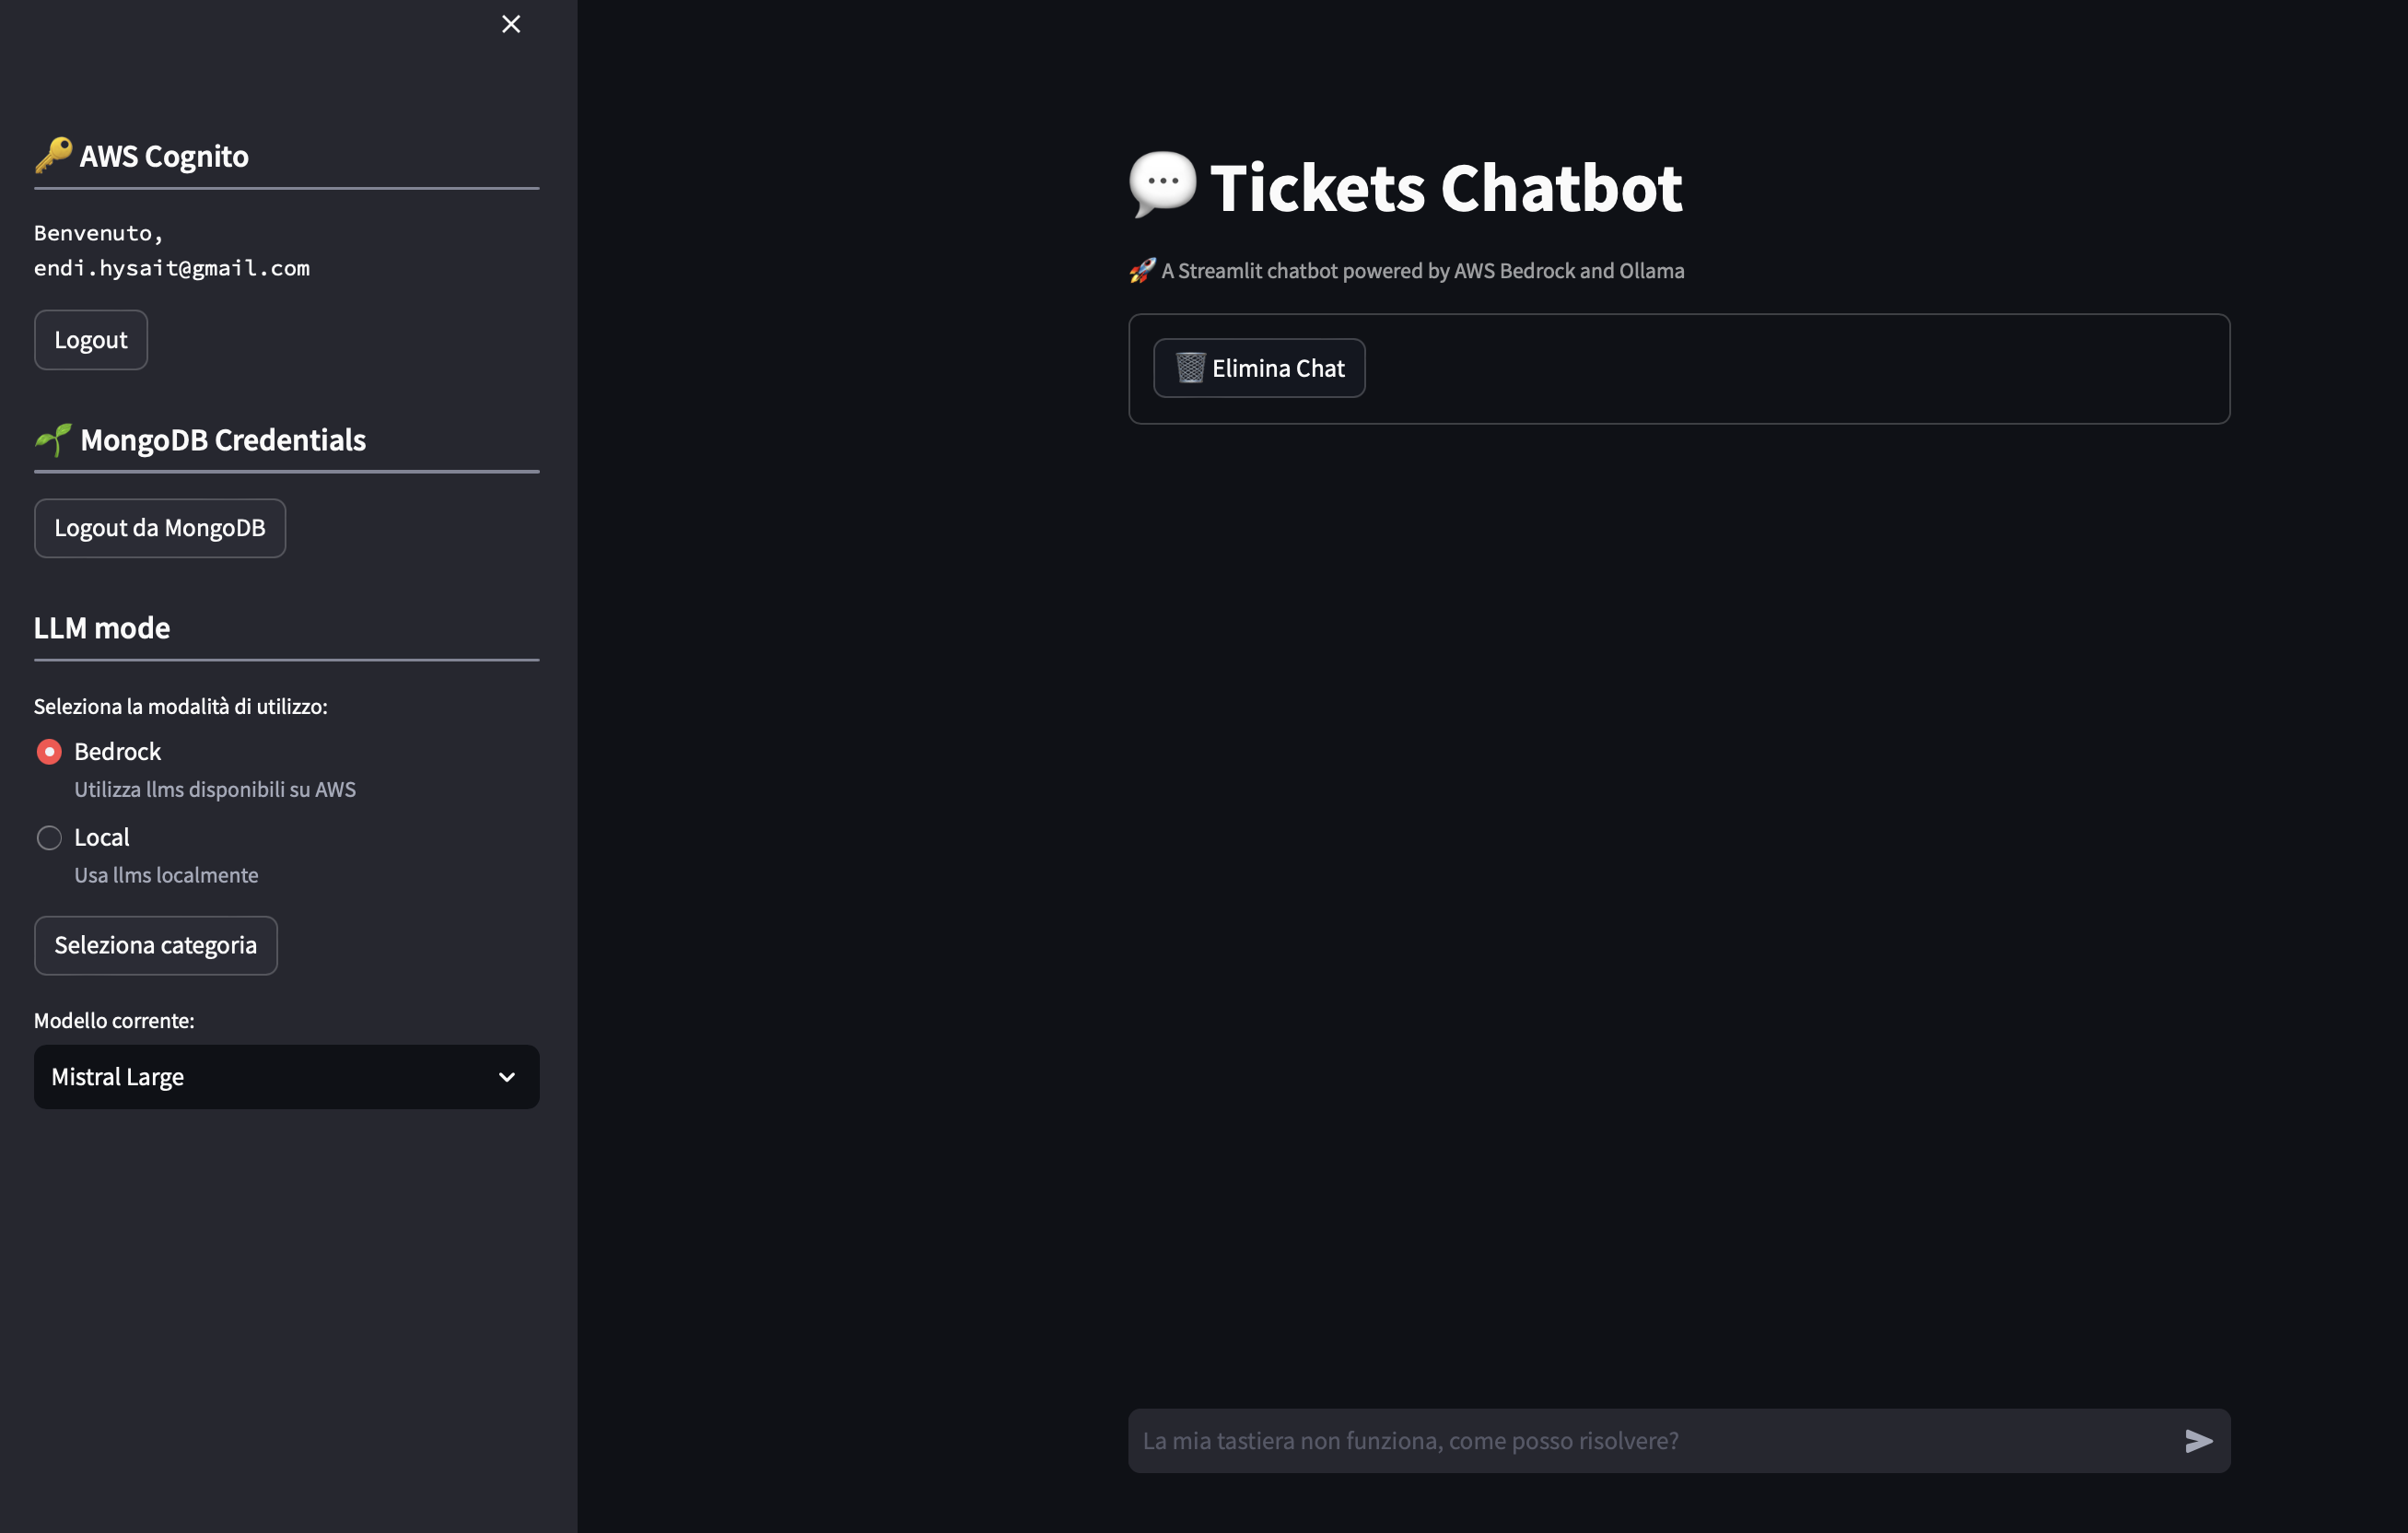
\includegraphics[width=0.85\textwidth]{afterMongoCredentials.png}
    \caption{Intefaccia del \textit{chatbot} }
    \label{fig:chatbot}
\end{figure}

\begin{figure} [H]
    \centering
    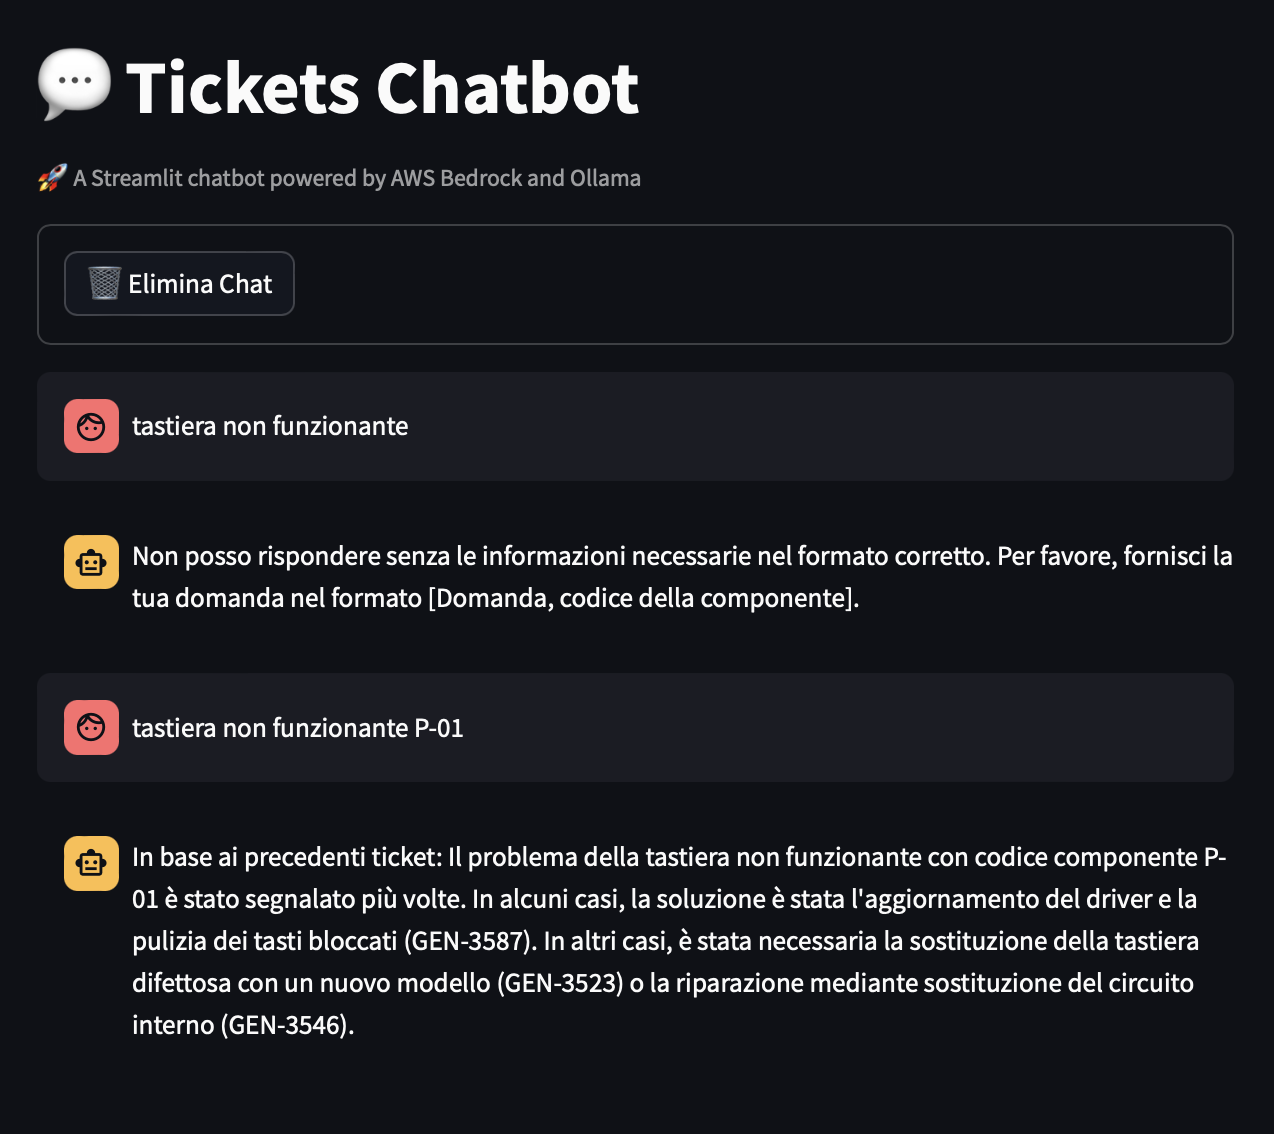
\includegraphics[width=0.85\textwidth]{chatExample.png}
    \caption{Proposta di risoluzione generata dal \textit{chatbot}}
    \label{fig:chatbotResponse}
\end{figure}

 \subsection{Copertura dei requisiti}
Il sistema di proposte di risoluzione Jira e il \textit{chatbot} coprono l'interezza dei requisiti descritti nella tabella \ref{tab:tracciamentoRequisiti}, garantendo che i prodotti sviluppati rispettassero le specifiche definite durante l' analisi e che soddisfasse le aspettative dell'azienda. Non avendo svolto dei \textit{test} codificati ma solo dei \textit{test} effettuati manualmente, non ho un valore di \textit{code coverage} che mi permetta di quantificare il numero di righe di codice coperte dai \textit{test}. La decisione di non svolgere dei \textit{test} codificati è stata dettata dalla necessità di concentrarmi sullo sviluppo dei progetti e di dimostrare la fattibilità e l'utilità dei prodotti sviluppati al termine delle otto settimane di \textit{stage}.

\subsection{Materiali prodotti}
Il mio periodo di \textit{stage} ha visto la produzione di diversi materiali al fine di documentare il lavoro svolto e le scelte progettuali fatte.
Di seguito la tabella riporta una valutazione quantitativa dell'esperienza di \textit{stage}, in base ai diversi aspetti considerati:
\begin{table}[H]
    \centering
    \begin{tabular}{|c|c|}
        \hline
        \multicolumn{2}{|c|}{\textbf{Documentale}} \\
        \hline
        Documenti & 2 \\
        \hline
        \textit{Sprint review} svolte & 8 \\
        \hline
        \multicolumn{2}{|c|}{\textbf{Tecnico}} \\
        \hline
        \textit{Handlers} implementati & 2 \\
        \hline
        \textit{Services} implementati & 9 \\
        \hline
        Interfacce & 14 \\
        \hline
        Classi implementate & 3 \\
        \hline
    \end{tabular}
    \caption{Materiali prodotti durante il periodo di \textit{stage}}
    \label{tab:quantitaMateriali}
\end{table}

